
\documentclass[11pt,a4paper]{article}

% Modelo institucional adaptado ao TP1 de Computação Gráfica
\usepackage[utf8]{inputenc}
\usepackage[T1]{fontenc}
\usepackage[brazilian]{babel}
\usepackage{geometry}
\geometry{a4paper,top=2.5cm,bottom=2.5cm,left=2.0cm,right=2.0cm}
\usepackage{amsmath,amssymb,amsfonts}
\usepackage{booktabs,tabularx,array}
\usepackage{graphicx}
\usepackage{xcolor}
\usepackage{enumitem}
\usepackage[most]{tcolorbox}
\usepackage{fancyhdr}
\usepackage{float}
\usepackage{caption}
\usepackage{subcaption}
\usepackage{microtype}
\usepackage[colorlinks=true,linkcolor=ufopred,citecolor=deepnavy,urlcolor=ufopred]{hyperref}

\definecolor{ufopred}{RGB}{140,29,36}
\definecolor{deepnavy}{RGB}{20,35,60}
\definecolor{lightgray}{RGB}{245,247,250}
\definecolor{darkslate}{RGB}{30,40,50}

\pagestyle{fancy}
\fancyhf{}
\setlength{\headheight}{14pt}
\rhead{\textcolor{darkslate}{\small \textbf{BCC327 -- Computação Gráfica}}}
\lhead{\textcolor{darkslate}{\small TP1 -- Árvores arteriais CCO}}
\cfoot{\thepage}
\tcbuselibrary{skins,breakable}
\setlength{\parskip}{0.25em}
\setlength{\parindent}{1.2em}
\captionsetup{font=small,labelfont=bf}
\graphicspath{{figures/}}

\begin{document}

% Título e identificação
\begin{center}
  {\large\textbf{UNIVERSIDADE FEDERAL DE OURO PRETO -- UFOP}}\\
  {\small Departamento de Computação -- DECOM\\
  Curso de Ciência da Computação}\\[0.55cm]
  {\LARGE\bfseries\textcolor{ufopred}{Visualização Geométrica e Rasterização de Árvores Arteriais CCO}}\\[0.35cm]
  {\large
  \textbf{Cauã Lemos Câmara},
  \textbf{César Augusto Tiago Totô} e
  \textbf{Roberto Antonino Menegassi Filho}}\\[0.15cm]
  {\small Disciplina: BCC327 -- Computação Gráfica \quad Semestre: 2026.2\\
  Docente: Prof. Dr. Rafael Alves Bonfim de Queiroz}
\end{center}

\begin{tcolorbox}[colback=lightgray,colframe=deepnavy,arc=3pt,title=\textbf{RESUMO},fonttitle=\bfseries]
\small
Este trabalho apresenta o desenvolvimento parcial de uma aplicação para visualização de árvores arteriais geradas pelo método \emph{Constrained Constructive Optimization} (CCO), utilizando modelos geométricos fornecidos em formato VTK. O objetivo foi desenvolver uma aplicação de Computação Gráfica que integre leitura, representação, transformação, rasterização e recorte de modelos CCO, destacando quais algoritmos clássicos foram implementados pelo grupo e quais foram delegados à biblioteca. A aplicação foi desenvolvida em Python com PyVista e reúne leitura dos dados, representação dos segmentos vasculares por tubos, codificação visual do raio, controles de câmera e projeção, preenchimento de polígono pelo algoritmo Scanline e seleção de técnicas de antialiasing disponibilizadas pela biblioteca. O modelo tridimensional \texttt{tree3D\_Nterm016.vtk} foi utilizado como exemplo principal. Para esse arquivo, foram identificados 32 pontos, 31 células lineares e raios entre 0,2261241 e 0,6870107. O preenchimento Scanline aplicado a um polígono côncavo de teste ocupou 216 dos 780 pixels da grade (27,7\%), conforme indicado pela própria execução. Os módulos de rasterização de linhas e de recorte de segmentos e polígonos permanecem sem implementação; além disso, o módulo de câmera oferece vistas predefinidas, mas não implementa controles próprios de translação, rotação e escala. Assim, o relatório distingue os recursos efetivamente implementados daqueles previstos no enunciado e ainda pendentes.
\vspace{0.15cm}

\textbf{Palavras-chave:} Computação Gráfica; PyVista; CCO; rasterização; Scanline; visualização 3D.
\end{tcolorbox}

\section{Introdução e objetivos}

Árvores arteriais podem ser representadas computacionalmente como estruturas ramificadas compostas por pontos, segmentos e atributos geométricos associados aos vasos. No contexto deste trabalho, os modelos foram gerados previamente pelo método \emph{Constrained Constructive Optimization} (CCO) e disponibilizados em arquivos VTK. O objetivo do TP1 não é reconstruir o método CCO, mas desenvolver uma aplicação que permita interpretar e visualizar seus resultados e exercitar conceitos fundamentais de Computação Gráfica.

A aplicação foi organizada em módulos Python e utiliza PyVista como interface de visualização sobre a infraestrutura VTK. O escopo efetivamente desenvolvido inclui a leitura dos modelos, a conversão de segmentos em tubos, a associação de cor e espessura ao raio, a seleção de vistas, a apresentação de uma região poligonal rasterizada por Scanline e a ativação de modos de antialiasing.

O objetivo geral deste artigo é documentar a arquitetura e os resultados observáveis da aplicação, com atenção à distinção entre algoritmos implementados pelo grupo e operações delegadas à biblioteca. Como objetivos específicos, busca-se: (i) ler e interpretar a estrutura geométrica dos modelos CCO (pontos, conectividade e raio); (ii) representar a árvore por tubos e codificar o raio por cor e/ou espessura; (iii) permitir vistas distintas do observador e a comparação entre projeção ortográfica e em perspectiva; (iv) implementar manualmente a rasterização de linhas (DDA e Bresenham) e de polígonos (Scanline); (v) comparar visualmente a renderização com e sem antialiasing; (vi) implementar o recorte de segmentos (Cohen-Sutherland e Liang-Barsky) e de polígonos (Sutherland-Hodgman); e (vii) documentar claramente o que foi implementado pelo grupo e o que foi realizado pela biblioteca.

O método CCO em si não foi reimplementado, os modelos foram fornecidos pelo professor.

\section{Fundamentação teórica}

\subsection{Modelos vasculares CCO e representação geométrica}

O método CCO é uma abordagem construtiva de otimização para geração de árvores vasculares, descrita por Schreiner e Buxbaum \cite{schreiner1993}. Neste TP1, os modelos CCO são dados de entrada fornecidos pelo docente. Portanto, a aplicação não executa o crescimento da árvore nem recalcula suas bifurcações: ela interpreta a geometria já armazenada no arquivo.

Os arquivos utilizados seguem o formato VTK \texttt{POLYDATA}. A estrutura contém coordenadas tridimensionais dos pontos, conectividade das células lineares e um atributo escalar denominado \texttt{raio}, armazenado por célula. Uma árvore pode, assim, ser tratada como um conjunto de vértices e arestas, em que cada aresta possui um raio associado. O número de pontos é obtido por \texttt{mesh.n\_points}, enquanto o número de células é obtido por \texttt{mesh.n\_cells}.

\subsection{Primitivas gráficas e codificação do raio}

Uma linha representa a conectividade entre dois pontos, mas pode ter pouca espessura visual. Para produzir uma representação volumétrica, o módulo 1 reconstrói cada segmento como uma linha independente e aplica o filtro \texttt{tube} do PyVista. O filtro gera uma superfície tubular ao redor da linha; no código, são solicitados oito lados e fechamento das extremidades (\texttt{capping=True}). A geração da superfície tubular é realizada pela biblioteca, não por um algoritmo de cilindrização implementado manualmente pelo grupo.

O raio é utilizado de duas maneiras independentes. Na codificação por cor, o valor de cada segmento é normalizado para o intervalo unitário:
\[
t=\frac{r-r_{\min}}{r_{\max}-r_{\min}}, \qquad 0\leq t\leq 1.
\]
A cor RGB é então definida por
\[
R=t,\qquad G=0{,}5,\qquad B=1-t.
\]
Dessa forma, valores menores de raio tendem ao azul e valores maiores tendem ao vermelho, enquanto o canal verde permanece constante. Na codificação por espessura, o raio de visualização é proporcional ao raio original, multiplicado por um fator de escala calculado a partir do comprimento da malha. Quando a opção é desativada, todos os segmentos recebem uma espessura visual constante baseada na média dos raios.

\subsection{Câmera, vistas e projeção}

A posição do observador determina como a geometria do mundo é apresentada na imagem. O espaço do mundo descreve as coordenadas dos objetos na cena; a transformação de visualização posiciona esses objetos em relação à câmera, definindo uma origem e orientações de referência para o observador. A projeção transforma as coordenadas no referencial da câmera em coordenadas de imagem.

Na projeção perspectiva, objetos mais distantes tendem a ocupar uma área menor na imagem. Na projeção ortográfica (ou paralela), linhas paralelas permanecem paralelas e o tamanho projetado não depende da distância à câmera. O módulo 2 oferece três posições predefinidas (\textit{yz}, \textit{xz} e \textit{xy}) e alterna o estado de projeção por meio das funções de câmera do PyVista. A rotação livre e o zoom também podem ser realizados pela interação padrão da janela de visualização.

\subsection{Rasterização de Linhas}
Rasterizar um segmento é escolher os pixels que melhor o aproximam. O \textbf{DDA - Digital Differential Analyzer} usa o passo $\text{passos} = \max (|\Delta x|,|\Delta y|)$ e incrementos $(\Delta x/\text{passos},\,\Delta y/\text{passos})$ em ponto flutuante, arredondando cada posição. O \textbf{algoritmo de Bresenham}~\cite{bresenham1965} usa apenas aritmética inteira. Para inclinação entre $0$ e $1$, mantém-se um parâmetro de decisão

\begin{equation}
p_{0} = 2\Delta y - \Delta x, \qquad
p_{k+1} = \begin{cases} p_k + 2\Delta y & \text{se } p_k<0 \;(\text{mantém } y)\\ p_k + 2(\Delta y-\Delta x) & \text{se } p_k\ge 0 \;(y\leftarrow y\pm1)\end{cases}
\end{equation}
e os demais octantes são tratados trocando os papéis de $x$ e $y$.

\subsection{Rasterização de polígonos: Scanline Fill}

Rasterizar um polígono significa determinar quais elementos de uma grade discreta pertencem ao seu interior. O Scanline Fill percorre a região linha a linha. Para cada coordenada vertical inteira, são calculadas as interseções da linha de varredura com as arestas não horizontais do polígono. As interseções são ordenadas pela coordenada horizontal e os pixels entre pares sucessivos são preenchidos, segundo a regra par--ímpar.

A implementação utiliza uma tabela de arestas (ET), organizada pela coordenada mínima $y$ de cada aresta, e uma tabela de arestas ativas (AET), atualizada a cada linha. A coordenada horizontal de cada interseção é atualizada incrementalmente por
\[
x_{k+1}=x_k+\frac{1}{m},
\]
em que $m$ é a inclinação da aresta. A implementação ignora arestas horizontais, remove arestas ao alcançar seu $y_{\max}$, ordena as interseções e preenche os intervalos delimitados por pares de interseções. O resultado é uma matriz binária: valor 1 para pixels preenchidos e 0 para pixels externos.

\subsection{Aliasing e antialiasing}

A rasterização de contornos inclinados pode produzir bordas visualmente serrilhadas, fenômeno conhecido como aliasing. Técnicas de antialiasing buscam reduzir esse efeito por meio de amostragem ou filtragem. O módulo 5 não implementa filtros próprios: ele oferece controles para desativar o antialiasing ou solicitar à biblioteca PyVista/VTK os modos MSAA, FXAA e SSAA. Assim, o trabalho demonstra a seleção dessas opções da API, sem apresentar uma implementação manual dos respectivos algoritmos.

\begin{table}[htbp]
\centering
\caption{Comparação entre as técnicas de antialiasing (MSAA, FXAA e SSAA)}
\label{tab:antialiasing}
\begin{tabular}{|l|p{5cm}|p{4.5cm}|}
\hline
\textbf{Técnica} & \textbf{Funcionamento} & \textbf{Qualidade}\\ \hline
\textbf{SSAA} \newline (Super Sampling) & Renderiza a cena em uma resolução superior (ex: 4x) e depois redimensiona para a resolução nativa da tela. & \textbf{Altíssima}: Suaviza geometria, texturas e efeitos de shader em toda a cena. \\ \hline
\textbf{MSAA} \newline (Multi-Sampling) & Amostra múltiplos pontos de cor e profundidade de forma seletiva, apenas nas \textit{bordas dos polígonos}. & \textbf{Boa}: Excelente para arestas geométricas, mas não afeta texturas ou pixels internos. \\ \hline
\textbf{FXAA} \newline (Fast Approximate) & Técnica de pós-processamento 2D que analisa a imagem já renderizada, deteta contrastes e desfoca as bordas. & \textbf{Aceitável}: Corrige o serrilhado de forma geral, mas pode causar um leve desfoque na imagem. \\ \hline
\end{tabular}
\end{table}


\subsection{Recorte de segmentos}
\textbf{Cohen-Sutherland.} Cada extremo recebe um código de 4 bits (esquerda, direita, abaixo, acima). Se $c_1\,|\,c_2=0$, o segmento é aceito; se $c_1\,\&\,c_2\neq0$, é rejeitado; caso contrário, um extremo externo é substituído pela interseção com a borda indicada, por exemplo
\begin{equation}
x = x_1 + (x_2-x_1)\,\frac{y_{\max}-y_1}{y_2-y_1},\quad y=y_{\max},
\end{equation}
e o processo se repete.

\textbf{Liang--Barsky}~\cite{liangbarsky1984}. Parametriza-se $P(t)=P_1+t(P_2-P_1)$, $t\in[0,1]$, e impõe-se $t\,p_k\le q_k$ para cada borda, com
$p=(-\Delta x,\Delta x,-\Delta y,\Delta y)$ e $q=(x_1-x_{\min},\,x_{\max}-x_1,\,y_1-y_{\min},\,y_{\max}-y_1)$. Para $p_k<0$ o segmento está entrando e $r_k=q_k/p_k$ atualiza $t_{\text{ent}}=\max(0,r_k)$; para $p_k>0$ está saindo e $t_{\text{sai}}=\min(1,r_k)$. Se $p_k=0$ e $q_k<0$, o segmento é paralelo e externo. O segmento é visível se $t_{\text{ent}}\le t_{\text{sai}}$.

\textbf{Cyru--Beck}~\cite{cyrusbeck1978} (apenas discutido). Generaliza o problema para qualquer janela \emph{convexa}: para cada aresta $i$ com normal externa $\mathbf n_i$ e ponto $\mathbf P_{E_i}$, impõe-se $\mathbf n_i\cdot(P(t)-\mathbf P_{E_i})\le0$, o que dá $p_i=\mathbf n_i\cdot\mathbf D$ e $q_i=\mathbf n_i\cdot(\mathbf P_{E_i}-\mathbf P_1)$, com $\mathbf D=P_2-P_1$. Liang--Barsky é a especialização desse esquema para retângulos alinhados aos eixos, onde os produtos escalares se reduzem a $\pm\Delta x$ e $\pm\Delta y$.

\subsection{Recorte de polígonos}
O algoritmo de \textbf{Sutherland--Hodgman}~\cite{sutherlandhodgman1974} recorta o polígono contra uma borda da janela por vez. Para cada aresta $(S,P)$ da lista de vértices, há quatro casos: (i) ambos dentro: emite $P$; (ii) $S$ dentro e $P$ fora: emite a interseção; (iii) ambos fora: nada; (iv) $S$ fora e $P$ dentro: emite a interseção e $P$. A saída de uma borda é a entrada da seguinte. O \textbf{Weiler--Atherton}~\cite{weileratherton1977} percorre os contornos do polígono e da janela alternando entre eles nos pontos de interseção, o que lhe permite produzir \emph{vários} polígonos de saída.

\section{Metodologia e arquitetura da aplicação}

\subsection{Tecnologias e organização}

A aplicação foi escrita em Python e utiliza PyVista para leitura dos arquivos VTK, construção de objetos geométricos, renderização e widgets de interação. NumPy é utilizado nas operações numéricas sobre os atributos e na construção da grade de pixels; Matplotlib fornece o objeto de mapa de cores RGB utilizado pelo módulo 1. O ponto de entrada é \texttt{main.py}, que instancia um \texttt{Plotter} com janela de 1920 por 1080 pixels e chama sequencialmente os módulos.

\begin{table}[H]
\centering
\small
\caption{Responsabilidade e situação dos módulos da aplicação.}
\label{tab:modulos}
\begin{tabularx}{\textwidth}{c l X l}
\toprule
\textbf{Módulo} & \textbf{Tema} & \textbf{Comportamento observado no código} & \textbf{Situação}\\
\midrule
1 & Leitura e atributos & Lê VTK, extrai pontos, células e raios; constrói tubos e controles de cor/espessura. & Implementado\\
2 & Câmera e vistas & Oferece três vistas predefinidas e alternância de projeção pela API. & Parcial\\
3 & Rasterização de linhas & A função \texttt{rasterizacao\_linhas} retorna sem executar algoritmo. & Implementado\\
4 & Rasterização de polígonos & Implementa ET/AET e preenchimento Scanline de polígono. & Implementado\\
5 & Antialiasing & Widgets selecionam opções MSAA, FXAA, SSAA ou desativação da API. & Via biblioteca\\
6 & Recorte de segmentos & A função \texttt{clipping\_line\_region} retorna sem executar algoritmo. & Implementado\\
7 & Recorte de polígonos & A função \texttt{clipping\_polygon\_region} retorna sem executar algoritmo. & Implementado\\
\bottomrule
\end{tabularx}
\end{table}

\subsection{Leitura e preparação dos modelos}

O módulo 1 carrega o arquivo informado na linha de comando ou, na ausência de argumento, utiliza \texttt{tree3D\_Nterm016.vtk}. O nome do atributo de raio é localizado procurando-se por nomes que contenham \texttt{raio}, \texttt{radius} ou \texttt{radii}. Os valores mínimo e máximo são calculados com NumPy. Em seguida, cada célula é percorrida para recuperar os pares de pontos consecutivos, associando-se a cada segmento o raio da célula de origem.

O código cria uma nova estrutura \texttt{PolyData} com linhas de dois pontos e replica o raio nos dois extremos de cada segmento. Essa estrutura é encaminhada ao filtro \texttt{tube}. A interface disponibiliza caixas de seleção independentes para ligar ou desligar o mapa de cores e a espessura proporcional ao raio.

\subsection{Câmera e interface}

O módulo 2 cria dois grupos de botões de opção. O primeiro altera a projeção por meio de \texttt{enable\_parallel\_projection()} e \texttt{disable\_parallel\_projection()}, o segundo seleciona as posições \texttt{yz}, \texttt{xz} e \texttt{xy}. A interação de mouse permanece sob responsabilidade do visualizador PyVista/VTK.

Foi identificada uma inconsistência que deve ser considerada na interpretação das capturas: no código fornecido, a opção rotulada como ``Projeção ortogonal'' chama \texttt{disable\_parallel\_projection()}, enquanto a opção rotulada como ``Projeção Paralela'' chama \texttt{enable\_parallel\_projection()}. Como a projeção paralela corresponde à ortográfica, os rótulos da interface estão invertidos em relação às chamadas realizadas. Por isso, o relatório não atribui o tipo de projeção apenas ao texto selecionado na captura.


\subsection{Rasterização de linhas}
Os algoritmos DDA e Bresenham foram implementados, ambos retornando a lista de pixels $(x,y)$ do segmento. A versão de Bresenham trata todos os octantes: quando $|\Delta x|\ge|\Delta y|$ avança-se em $x$, e caso contrário em $y$, ajustando os sinais dos passos. Os pontos da árvore são levados à grade inteira por $\lceil 500\,c\rceil$ por coordenada, e os 20 primeiros segmentos são rasterizados. A figura de comparação marca os pixels de Bresenham (células coloridas), os centros dos pixels do DDA (círculos) e a reta ideal contínua (tracejada).

\subsection{Rasterização de polígonos}
Cada segmento da árvore é transformado em um retângulo de 4 vértices: dada a direção unitária $\mathbf d$ do segmento e sua normal $\mathbf n$, os vértices são $P_1\mp\mathbf n h$ e $P_2\pm\mathbf n h$ (com as pontas estendidas em $h$ para evitar buracos nas junções), onde a meia-largura $h$ é proporcional ao raio, com mínimo de 1 pixel. Os polígonos são projetados para um buffer de $400\times400$ pixels (o centro do modelo vai para o meio da imagem) e preenchidos com o Scanline (ET, AET e regra par-ímpar), com a cor definida pela mesma regra do Módulo 1. Os vasos são ordenados por profundidade $z$ (e, em empate, do maior para o menor raio) antes do desenho, aproximando o algoritmo do pintor. O módulo também implementa uma rotação do modelo em torno de seu centro (eixo $Y$ em 3D e eixo $Z$ em 2D) antes da projeção. O buffer é exibido como uma malha de pixels (\texttt{ImageData}) ao lado da árvore e pode ser ocultado por um botão.

\subsection{Antialiasing}
Um grupo de botões de rádio permite alternar entre ausência de antialiasing, MSAA, FXAA e SSAA, que são implementados pelo pipeline gráfico do VTK e acionados via \texttt{enable\_anti\_aliasing} do PyVista. Este módulo não implementa os algoritmos, sua contribuição é a comparação interativa e a explicação do seu funcionamento.

\subsection{Recorte de segmentos}
Cohen-Sutherland e Liang-Barsky foram implementados manualmente, ambos retornando se o segmento é visível e seus extremos recortados. Contadores registram o número de interseções e de divisões realizadas, para a comparação entre os métodos. A janela de recorte é um retângulo centrado na árvore, com tamanho controlado por um \emph{slider} (de 10\% a 120\% da extensão do modelo; padrão de 50\%). O recorte opera no plano $xy$, em modelos 3D, o valor de $z$ dos novos extremos é obtido por interpolação linear ao longo do segmento original. A cena exibe a janela (laranja), as partes mantidas (verde) e as descartadas (vermelho), e um painel com o total de segmentos aceitos inteiros, cortados e rejeitados. Há também a geração de uma figura com três painéis (antes, depois com Cohen-Sutherland e depois com Liang-Barsky).

\subsection{Recorte de polígonos}
O Sutherland-Hodgman foi implementado para janelas retangulares alinhadas aos eixos, em quatro funções. \texttt{is\_inside} testa o semiplano de cada borda, considerando pontos sobre a borda como internos. \texttt{compute\_intersection} calcula o ponto de cruzamento por parametrização da aresta e, se ela é paralela à borda, devolve o ponto inicial. \texttt{sutherland\_hodgman\_clip\_edge} realiza um passo do algoritmo: percorre os vértices tomando o último como ``anterior'' do primeiro e aplica os quatro casos da Seção~2. Por fim, \texttt{sutherland\_hodgman\_clip} encadeia as quatro bordas na ordem \emph{abaixo, direita, topo, esquerda}, a saída de cada etapa servindo de entrada da seguinte, e devolve também o histórico do polígono após cada borda. Cada etapa percorre a lista uma única vez, portanto o custo é linear no número de vértices.

O polígono de teste usado na demonstração é \textbf{convexo}, com 7 vértices: $(-7,-2)$, $(-3,-6)$, $(4,-6)$, $(8,-1)$, $(6,5)$, $(0,8)$ e $(-5,6)$. Ele fica na constante \texttt{POLIGONO\_TESTE}, o que permite trocá-lo por qualquer outra lista de vértices. A janela de recorte tem tamanho fixo de $10\times8$, inicialmente centrada em $(3{,}5;\,2{,}5)$, e é \textbf{arrastada com o botão esquerdo do mouse}: observadores do VTK tratam os eventos de pressionar, mover e soltar, e as coordenadas de tela são convertidas para o mundo por \texttt{DisplayToWorld}. O centro é limitado a $[-15,15]\times[-11,11]$ para a janela não sair da cena.

A cena é 2D, com projeção paralela, câmera sobre o eixo $z$ e estilo de interação de imagem (sem rotação, apenas zoom). O polígono original é desenhado em cinza, a janela em preto e a saída do algoritmo em vermelho, em três níveis de $z$ ligeiramente diferentes para evitar sobreposição visual. A cada movimento da janela o recorte é recalculado sobre o polígono inteiro, e a saída só é desenhada se tiver pelo menos 3 vértices.

\section{Resultados}

Nos testes foram utiliza dois modelos de árvore tree2D\_Nterm128.vtk e tree3D\_Nterm016.vtk.

\subsection{Leitura e representação do modelo}
A Tabela~\ref{tab:modelo} resume o modelo utilizado nos testes e a Figura ~\ref{fig:comparacao_arvores} mostra as árvore representadas por tubos.

\begin{table}[!h]
  \centering\small
  \caption{Características do modelo CCO utilizado.}
  \label{tab:modelo}
  \begin{tabular}{ll}
    \toprule
    \textbf{Atributo} & \textbf{Valor}\\
    \midrule
    Arquivo & tree2D\_Nterm128.vtk\\
    Dimensão & 2D\\
    Número de pontos & 256\\
    Número de segmentos & 255\\
    Raio mínimo & 0.1454243\\
    Raio máximo & 1.1929671\\
    \bottomrule
  \end{tabular}
\end{table}

\begin{figure}[H]
    \centering
    % --- Primeira linha ---
    \begin{subfigure}{0.48\textwidth}
        \centering
        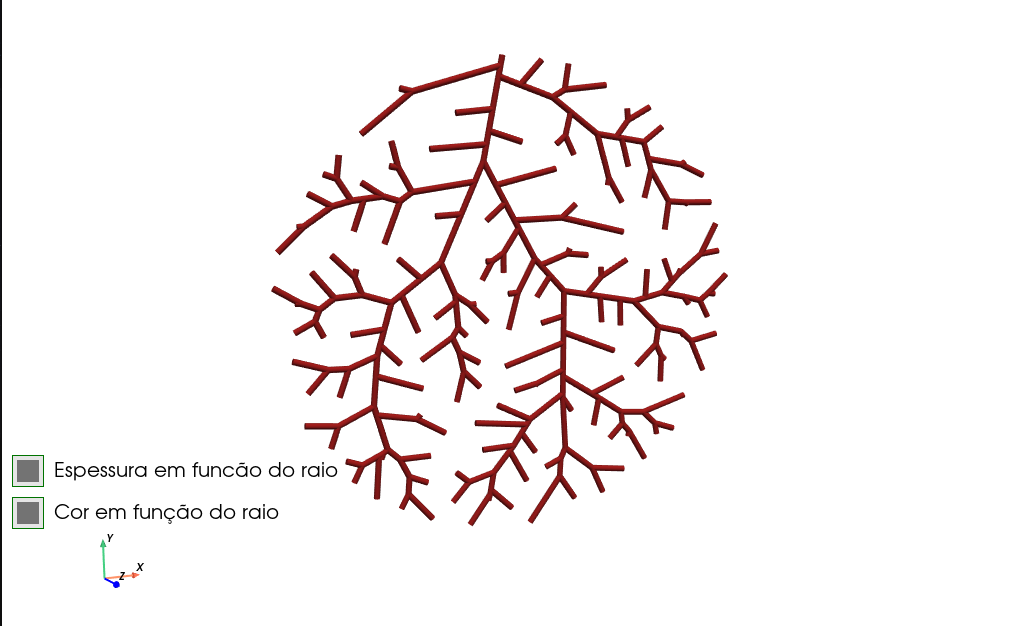
\includegraphics[width=\linewidth]{figures/desligado.png}
        \caption{Árvore com espessura desligada.}
        \label{fig:espessura}
    \end{subfigure}
    \hfill % Adiciona espaço horizontal entre as duas figuras
    \begin{subfigure}{0.48\textwidth}
        \centering
        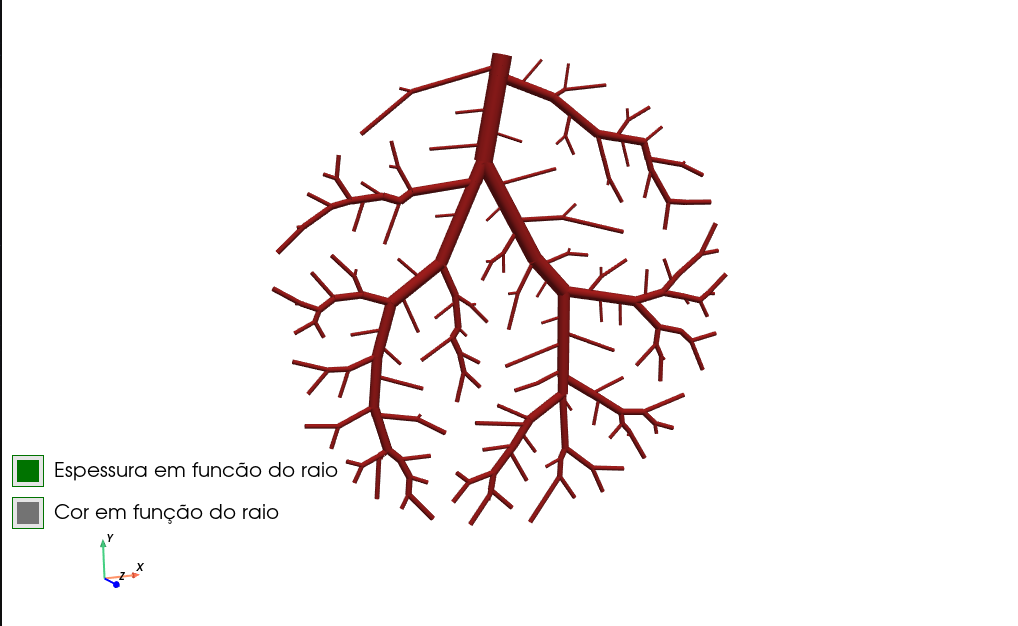
\includegraphics[width=\linewidth]{figures/espessura.png}
        \caption{Árvore com espessura relacionada ao raio.}
        \label{fig:espessura_raio}
    \end{subfigure}

    \vspace{1em} % Espaço vertical entre a primeira e a segunda linha

    % --- Segunda linha ---
    \begin{subfigure}{0.48\textwidth}
        \centering
        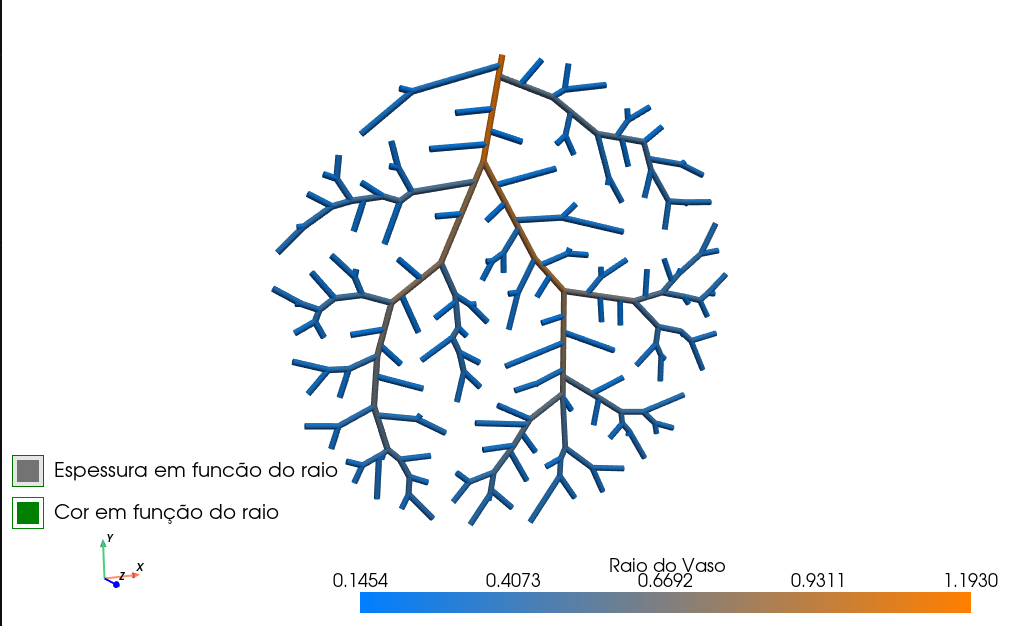
\includegraphics[width=\linewidth]{figures/cor.png}
        \caption{Árvore com espessura relacionada com a cor.}
        \label{fig:espessura_cor}
    \end{subfigure}
    \hfill
    \begin{subfigure}{0.48\textwidth}
        \centering
        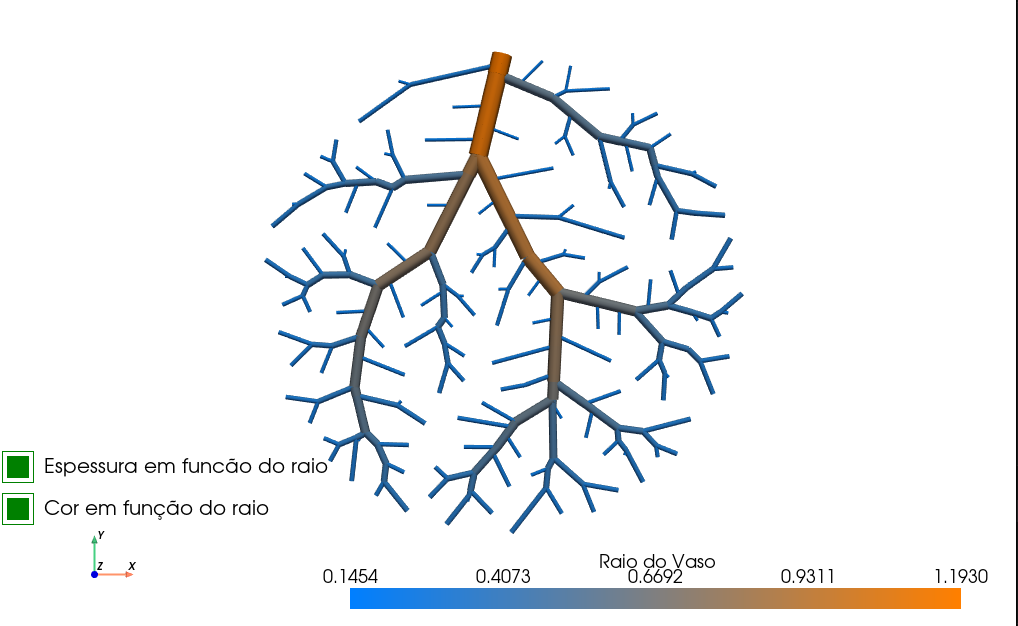
\includegraphics[width=\linewidth]{figures/cor_espessura.png}
        \caption{Árvore com espessura relacionada à cor e ao raio.}
        \label{fig:cor_raio}
    \end{subfigure}

    \caption{Comparação das diferentes configurações da árvore.}
    \label{fig:comparacao_arvores}
\end{figure}

\subsection{Modelo utilizado e atributos}

O modelo de exemplo é \texttt{tree3D\_Nterm016.vtk}. A leitura direta do arquivo e a informação apresentada pela aplicação indicam 32 pontos e 31 células lineares. O atributo \texttt{raio} possui mínimo de 0,2261241 e máximo de 0,6870107. Esses valores são reproduzidos na interface durante a execução (Figura~\ref{fig:app}).

\begin{figure}[H]
\centering
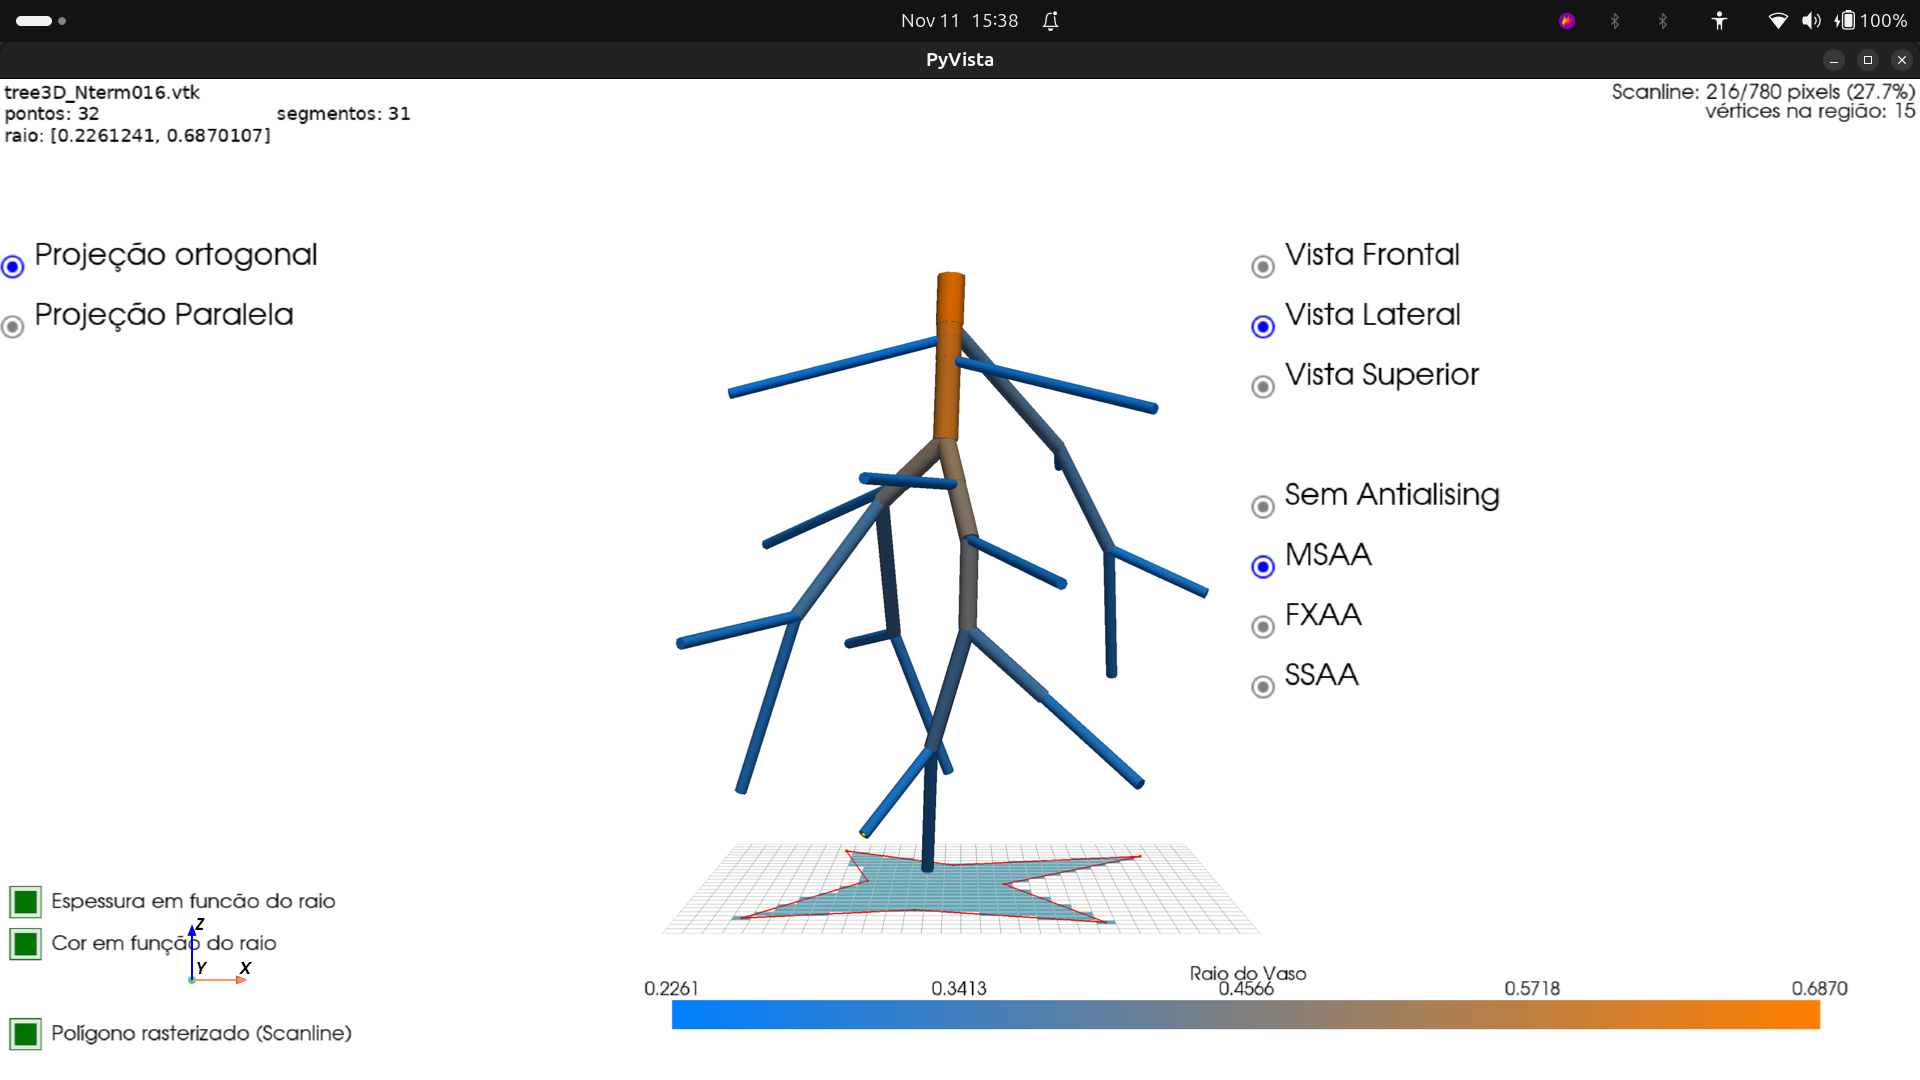
\includegraphics[width=0.94\textwidth]{figures/aplicacao_modelo_3d.png}
\caption{Aplicação em execução com o modelo \texttt{tree3D\_Nterm016.vtk}, mostrando os dados de entrada, a árvore tubular, os controles de câmera, antialiasing e atributos visuais.}
\label{fig:app}
\end{figure}

A Figura~\ref{fig:refcomp} compara a imagem de referência fornecida pelo docente para o mesmo conjunto com uma captura da aplicação. A comparação é qualitativa: ambas apresentam a estrutura ramificada, mas a aplicação adiciona controles interativos e a codificação visual pelo atributo de raio.

\begin{figure}[H]
\centering
\begin{subfigure}[t]{0.38\textwidth}
\centering
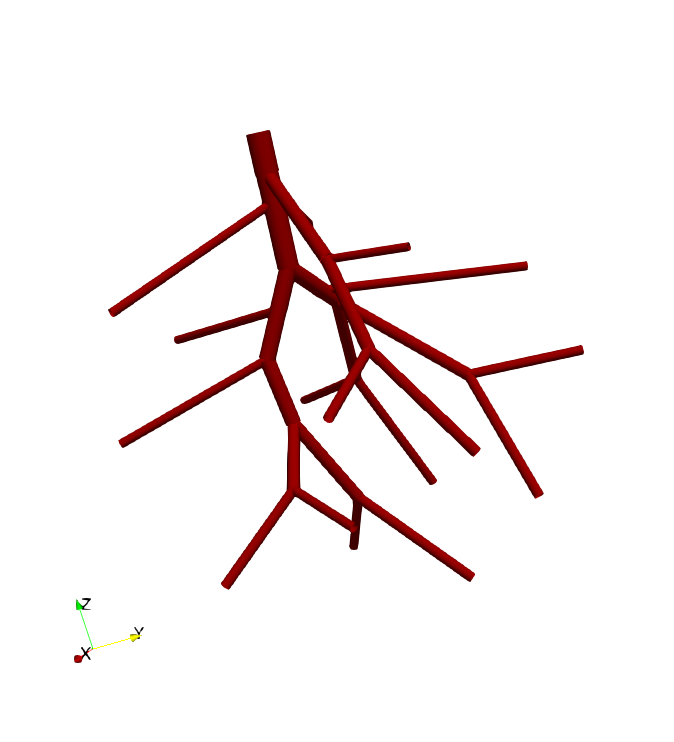
\includegraphics[height=5.4cm,keepaspectratio]{figures/tree3D_Nterm016_tube_solid.png}
\caption{Imagem de referência do docente.}
\end{subfigure}\hfill
\begin{subfigure}[t]{0.58\textwidth}
\centering
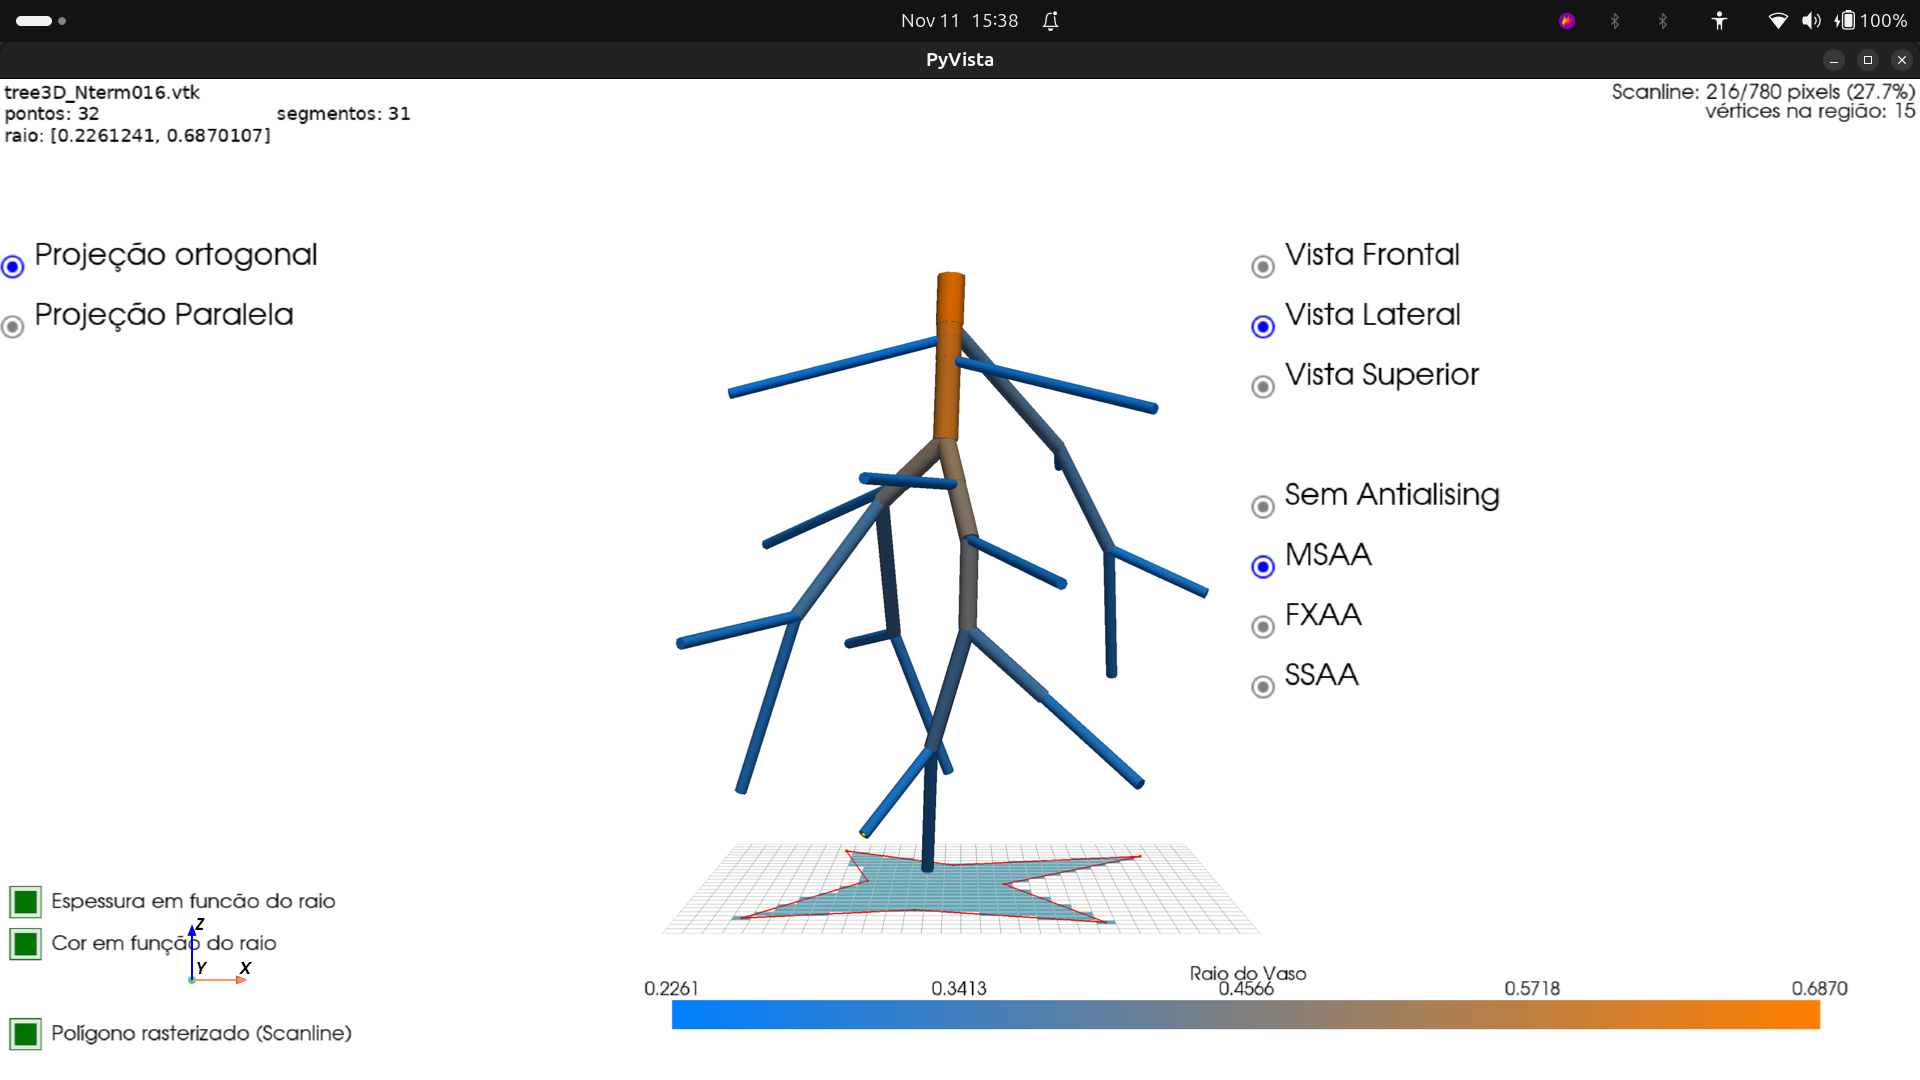
\includegraphics[width=\textwidth]{figures/aplicacao_modelo_3d.png}
\caption{Visualização produzida pela aplicação.}
\end{subfigure}
\caption{Comparação qualitativa do modelo tridimensional com a referência disponibilizada.}
\label{fig:refcomp}
\end{figure}

Na Figura \ref{fig:comparacao_vista} mostra a comparação da visualização da árvore ao mudar a câmera de posição.

\begin{figure}[H]
    \centering
    % --- Primeira linha ---
    \begin{subfigure}{0.48\textwidth}
        \centering
        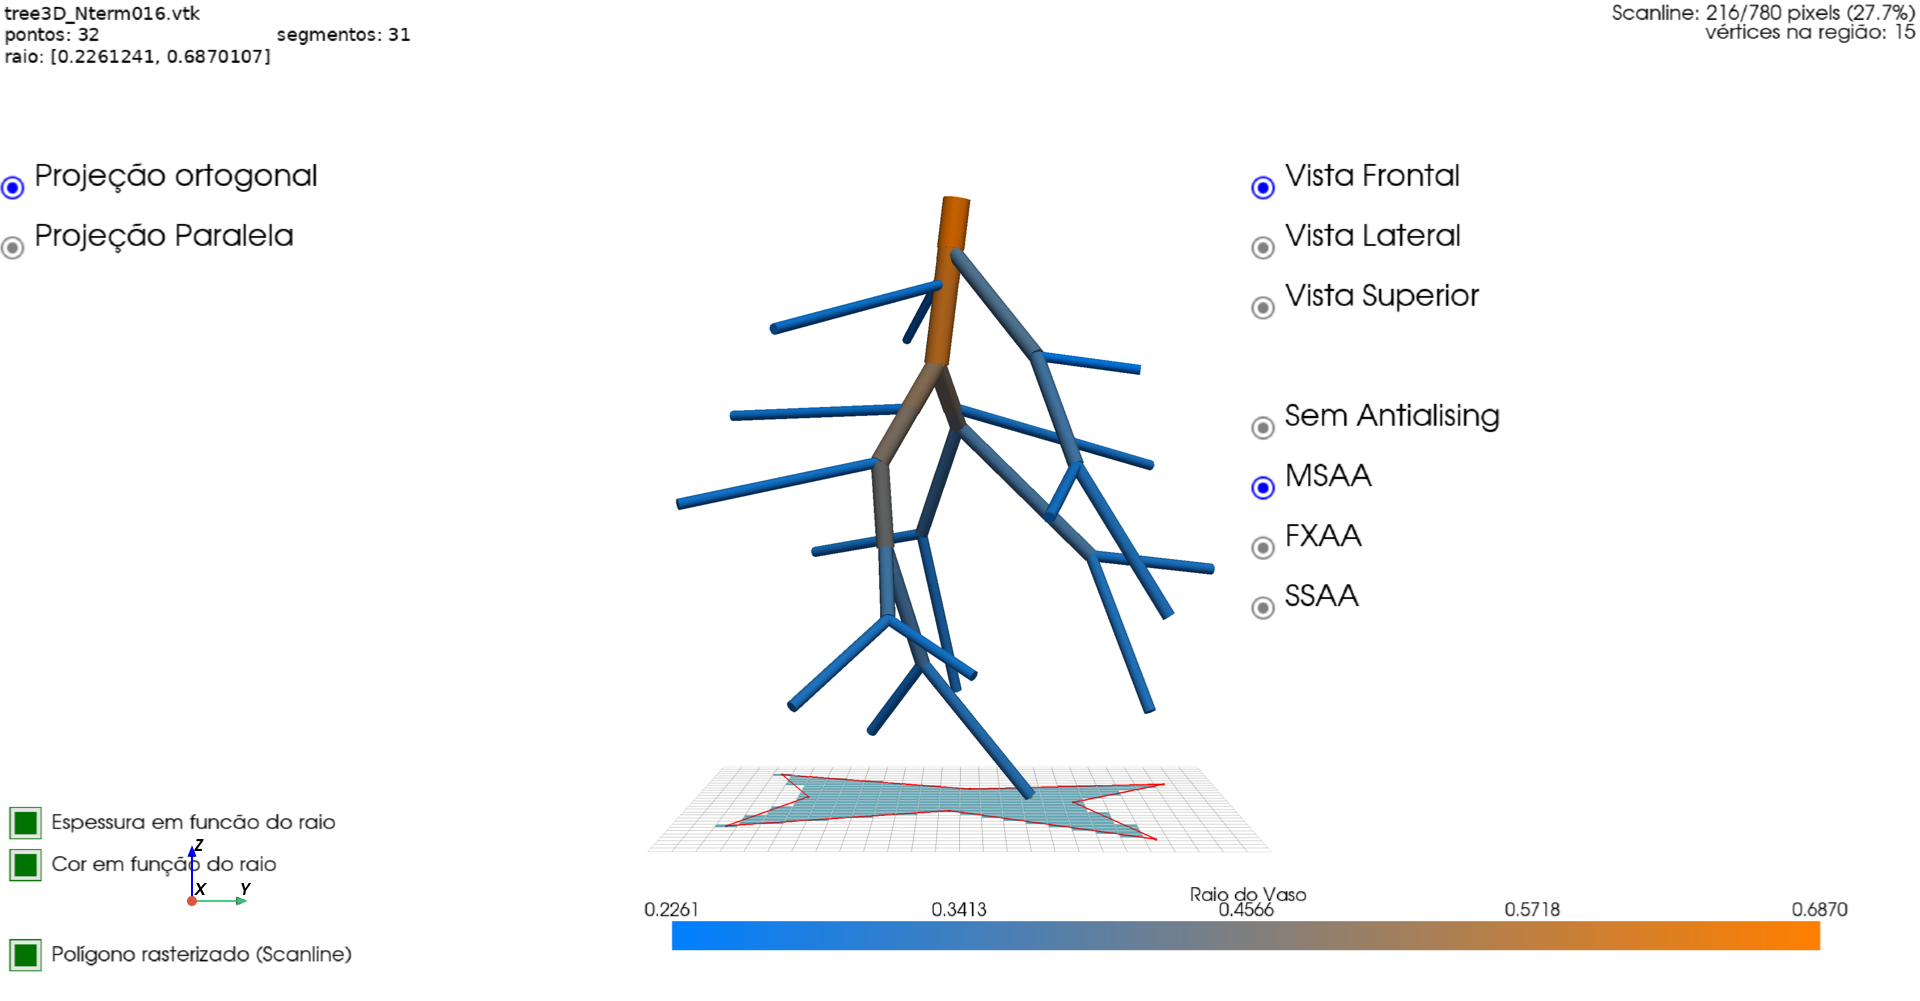
\includegraphics[width=\linewidth]{figures/vista_frontal.png}
        \caption{Frontal.}
        \label{fig:frontal}
    \end{subfigure}
    \hfill % Adiciona espaço horizontal entre as duas figuras
    \begin{subfigure}{0.48\textwidth}
        \centering
        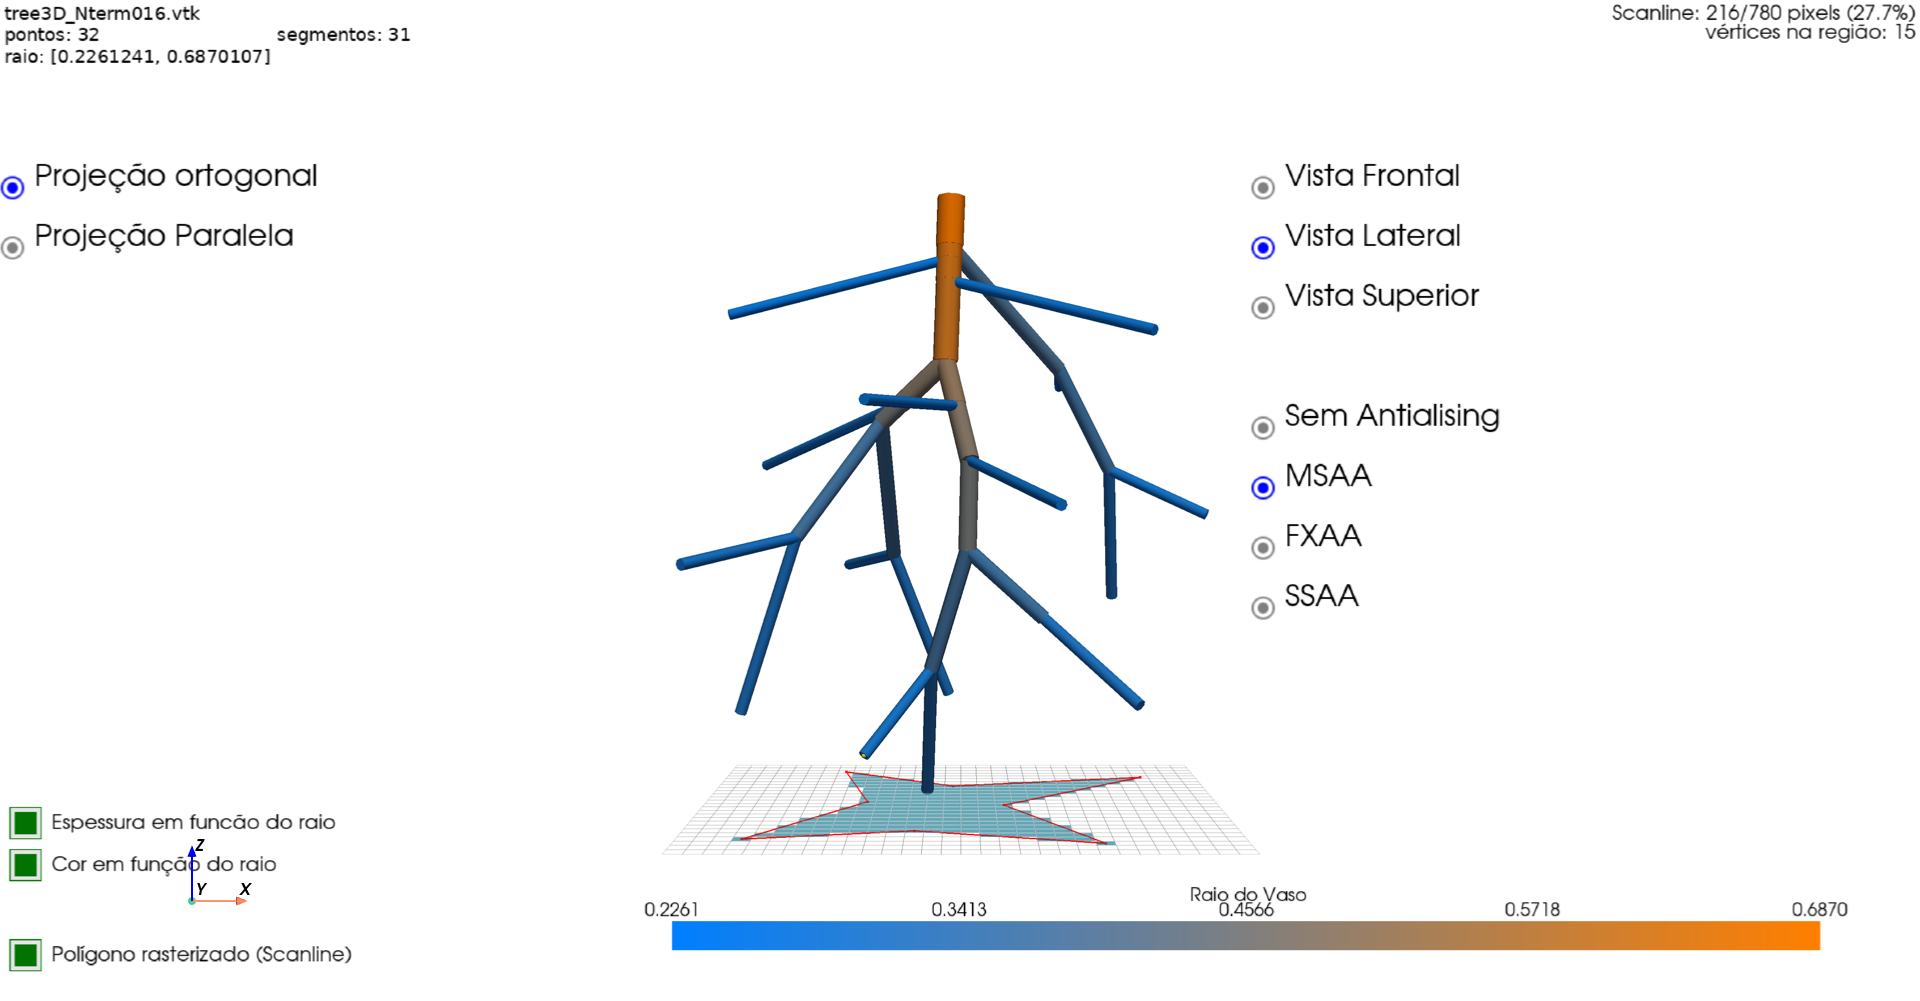
\includegraphics[width=\linewidth]{figures/vista_lateral.png}
        \caption{Lateral.}
        \label{fig:lateral}
    \end{subfigure}

    \vspace{1em} % Espaço vertical entre a primeira e a segunda linha

    % --- Segunda linha ---
    \begin{subfigure}{0.48\textwidth}
        \centering
        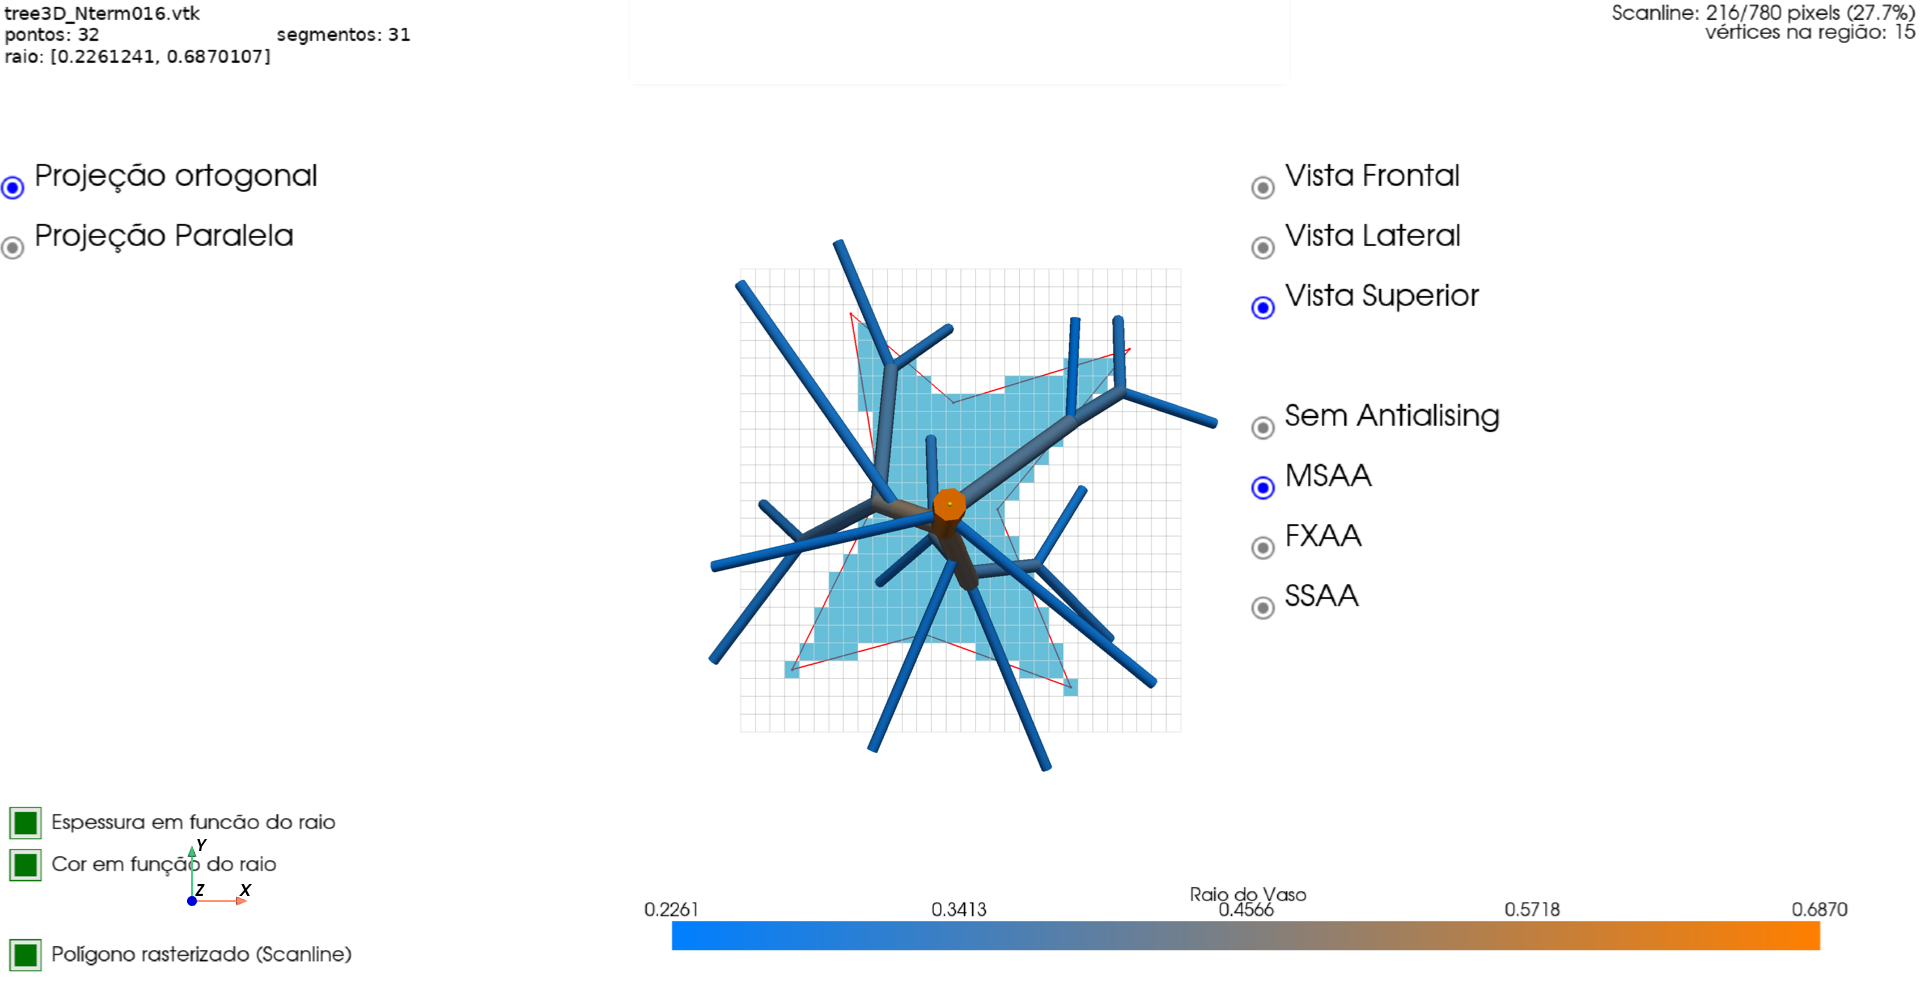
\includegraphics[width=\linewidth]{figures/vista_superior.png}
        \caption{Superior.}
        \label{fig:superior}
    \end{subfigure}

    \caption{Comparação da visualização da árvore ao mudar a posição da câmera.}
    \label{fig:comparacao_vista}
\end{figure}


\subsection{Rasterização de linhas}

Na Figura \ref{fig:rasterizacaoLinha} mostra a imagem gerada pela execução do algoritmo de Rasterização de Linha DDA e Bresenham.
\begin{figure}[H]
    \centering
    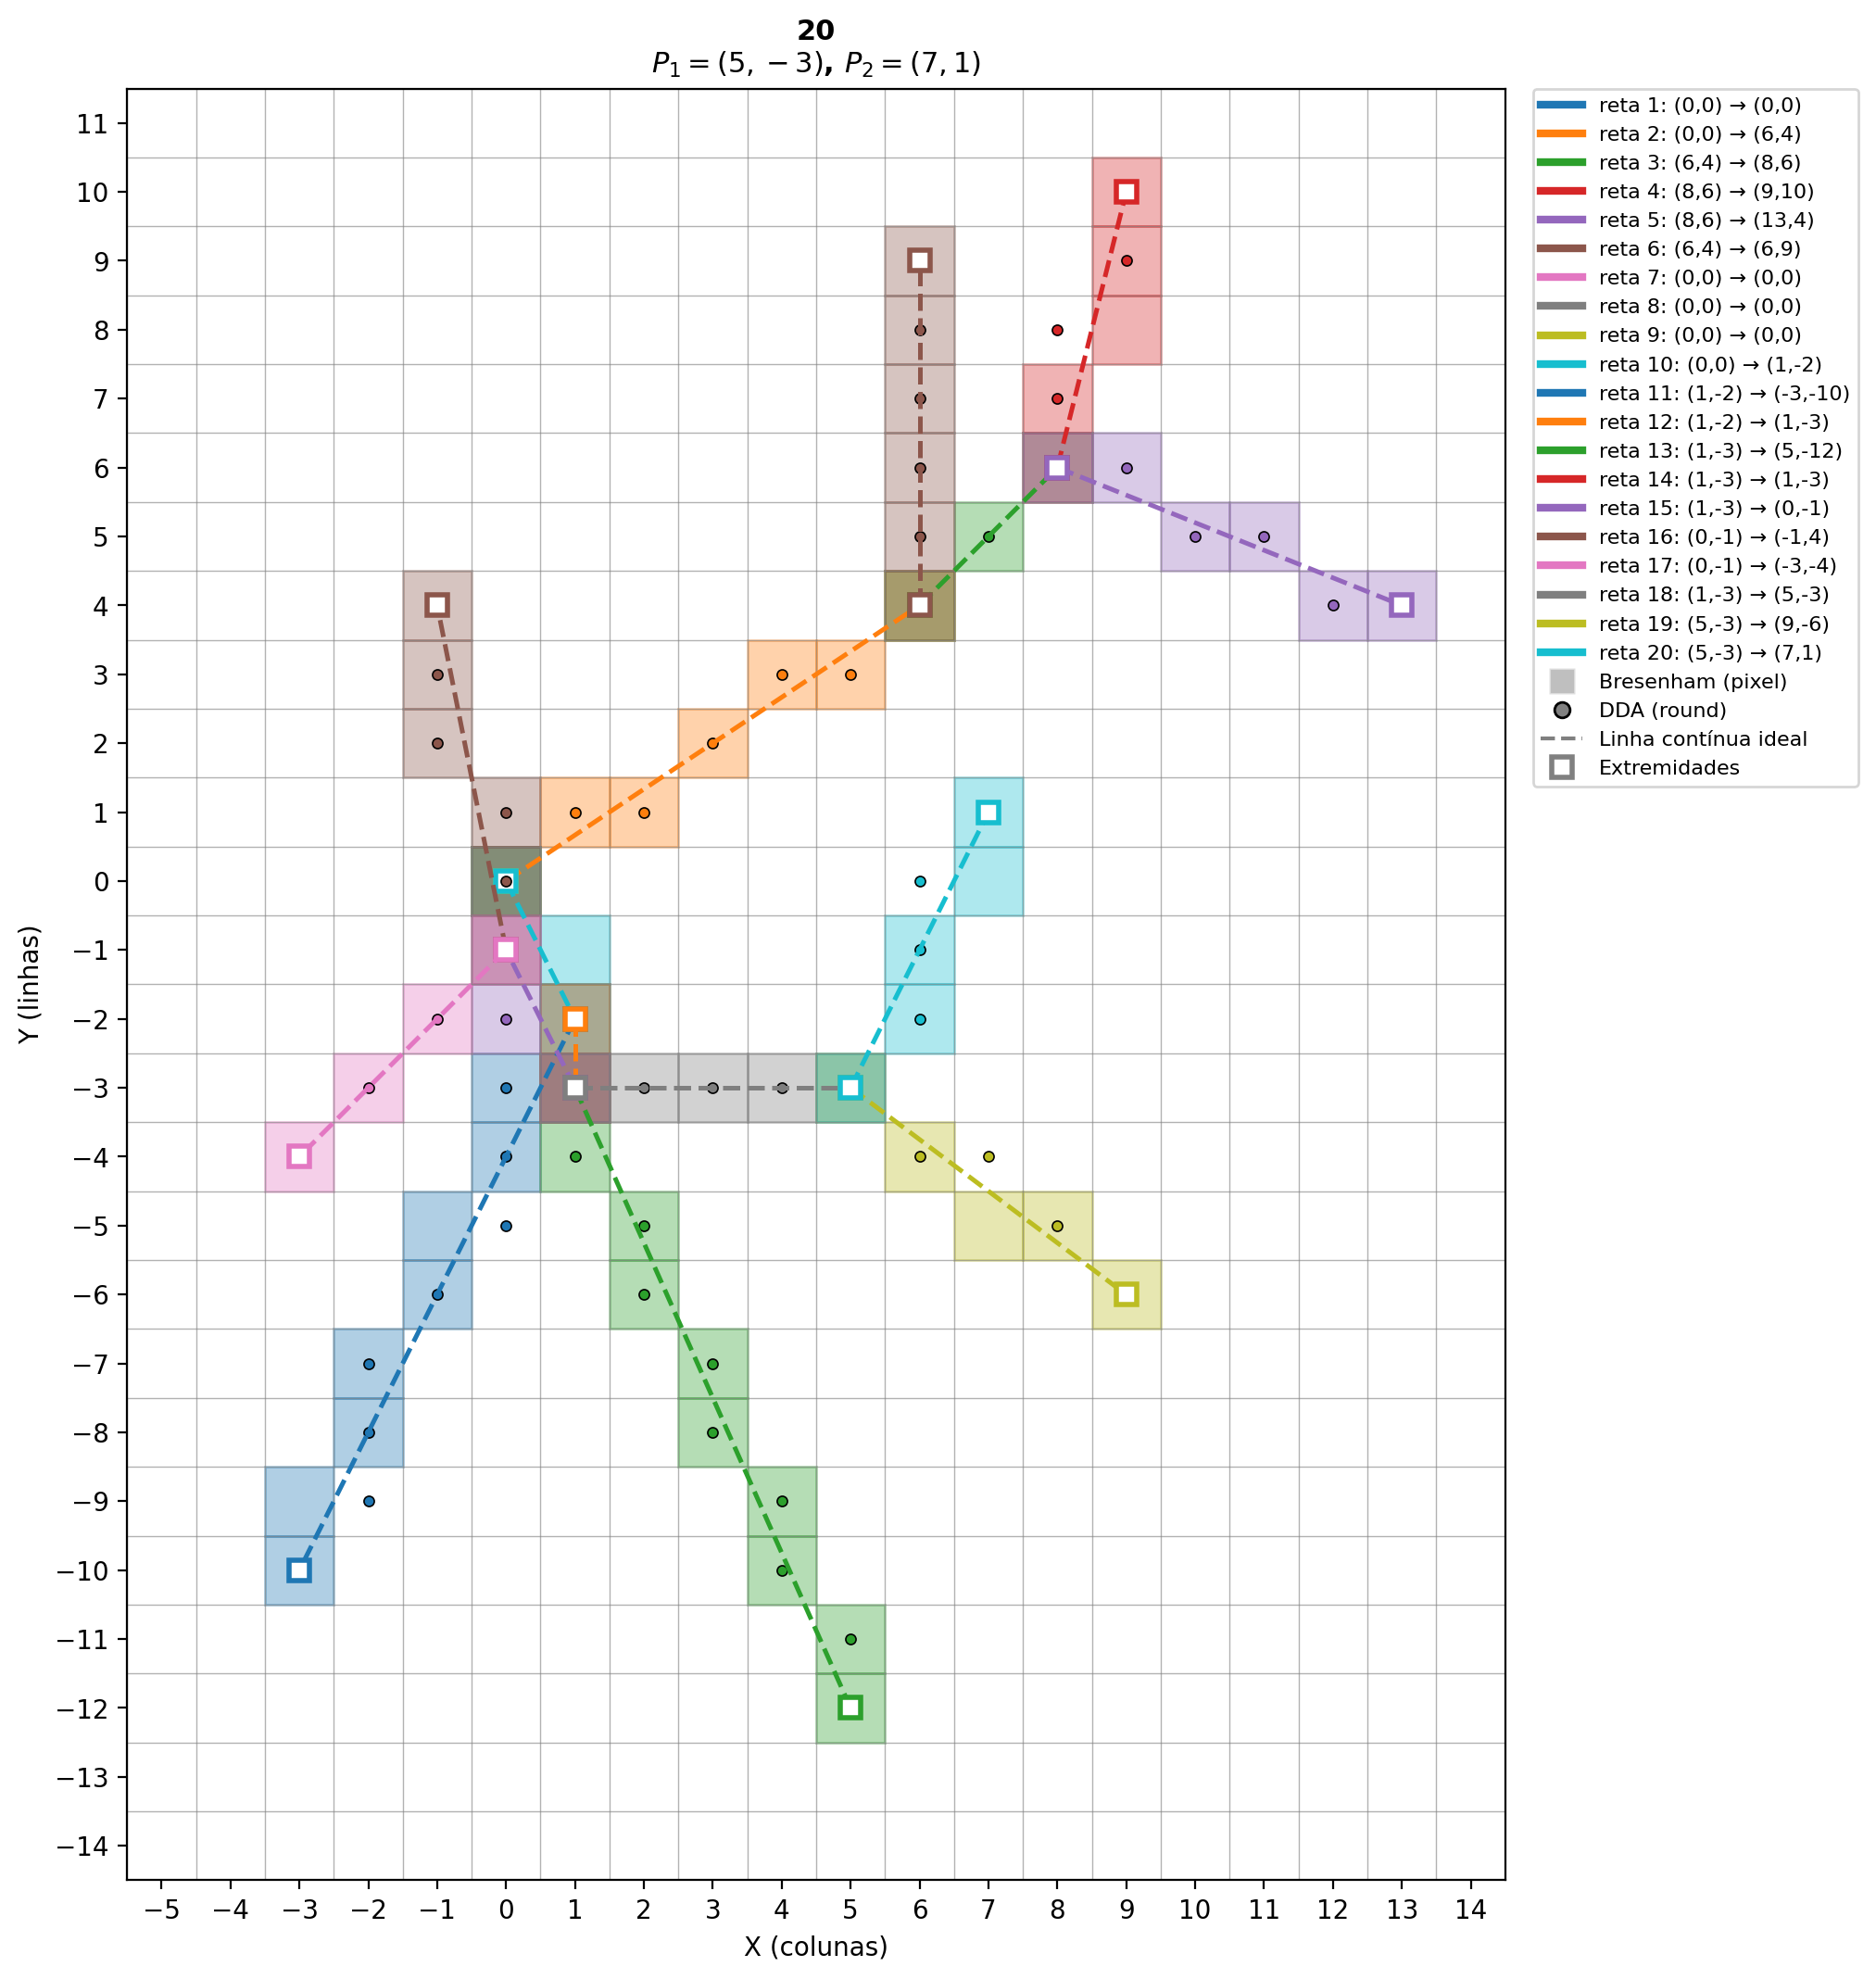
\includegraphics[width=1.0\linewidth]{figures/rasterizacao_linhas.png}
    \caption{Rasterização de Linhas.}
    \label{fig:rasterizacaoLinha}
\end{figure}

\subsection{Rasterização de polígonos}
Na Figura \ref{fig:comparacao_arvores_rasterizacao} mostra a comparação da rasterização de polígono (algoritmo Scanline) da árvore em dimensões diferentes do modelo do arquivo treexD\_Nterm128.vtk. A árvore a direita em azul é a árvore rasterizada.
\begin{figure}[H]
    \centering
    \begin{subfigure}{0.48\textwidth}
        \centering
        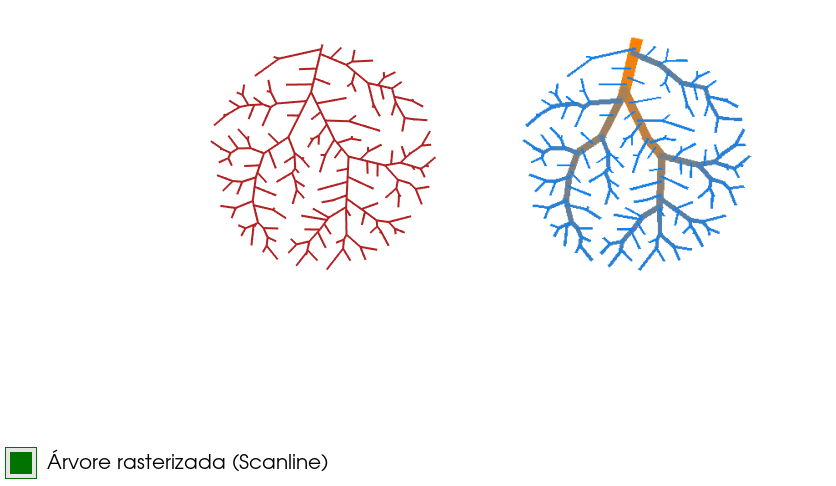
\includegraphics[width=\linewidth]{figures/rasterizacaoPligono_2D.png}
        \caption{Rasterização de Polígono em Árvore 2D.}
        \label{fig:rasteriza2D}
    \end{subfigure}
    \hfill % Adiciona espaço horizontal entre as duas figuras
    \begin{subfigure}{0.48\textwidth}
        \centering
        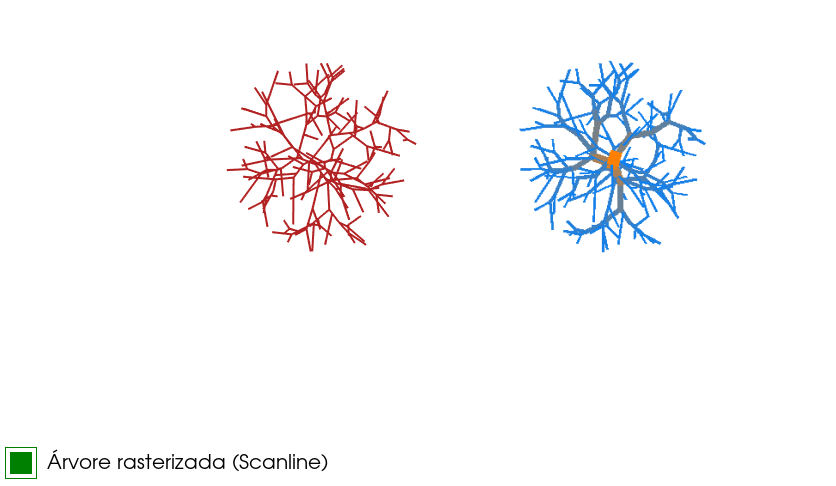
\includegraphics[width=\linewidth]{figures/rasterizacaoPoligono_3D.png}
        \caption{Rasterização de Polígono em Árvore 3D.}
        \label{fig:rasteriza3D}
    \end{subfigure}

    \caption{Comparação de Rasterização em diferentes dimensões de árvore.}
    \label{fig:comparacao_arvores_rasterizacao}
\end{figure}

\subsection{Antialiasing}
Na figura \ref{fig:comparacao_arvores_antiliasing} mostra a alternância entre ausência de antialiasing, MSAA, FXAA e SSAA.

\begin{figure}[H]
    \centering
    % --- Primeira linha ---
    \begin{subfigure}{0.48\textwidth}
        \centering
        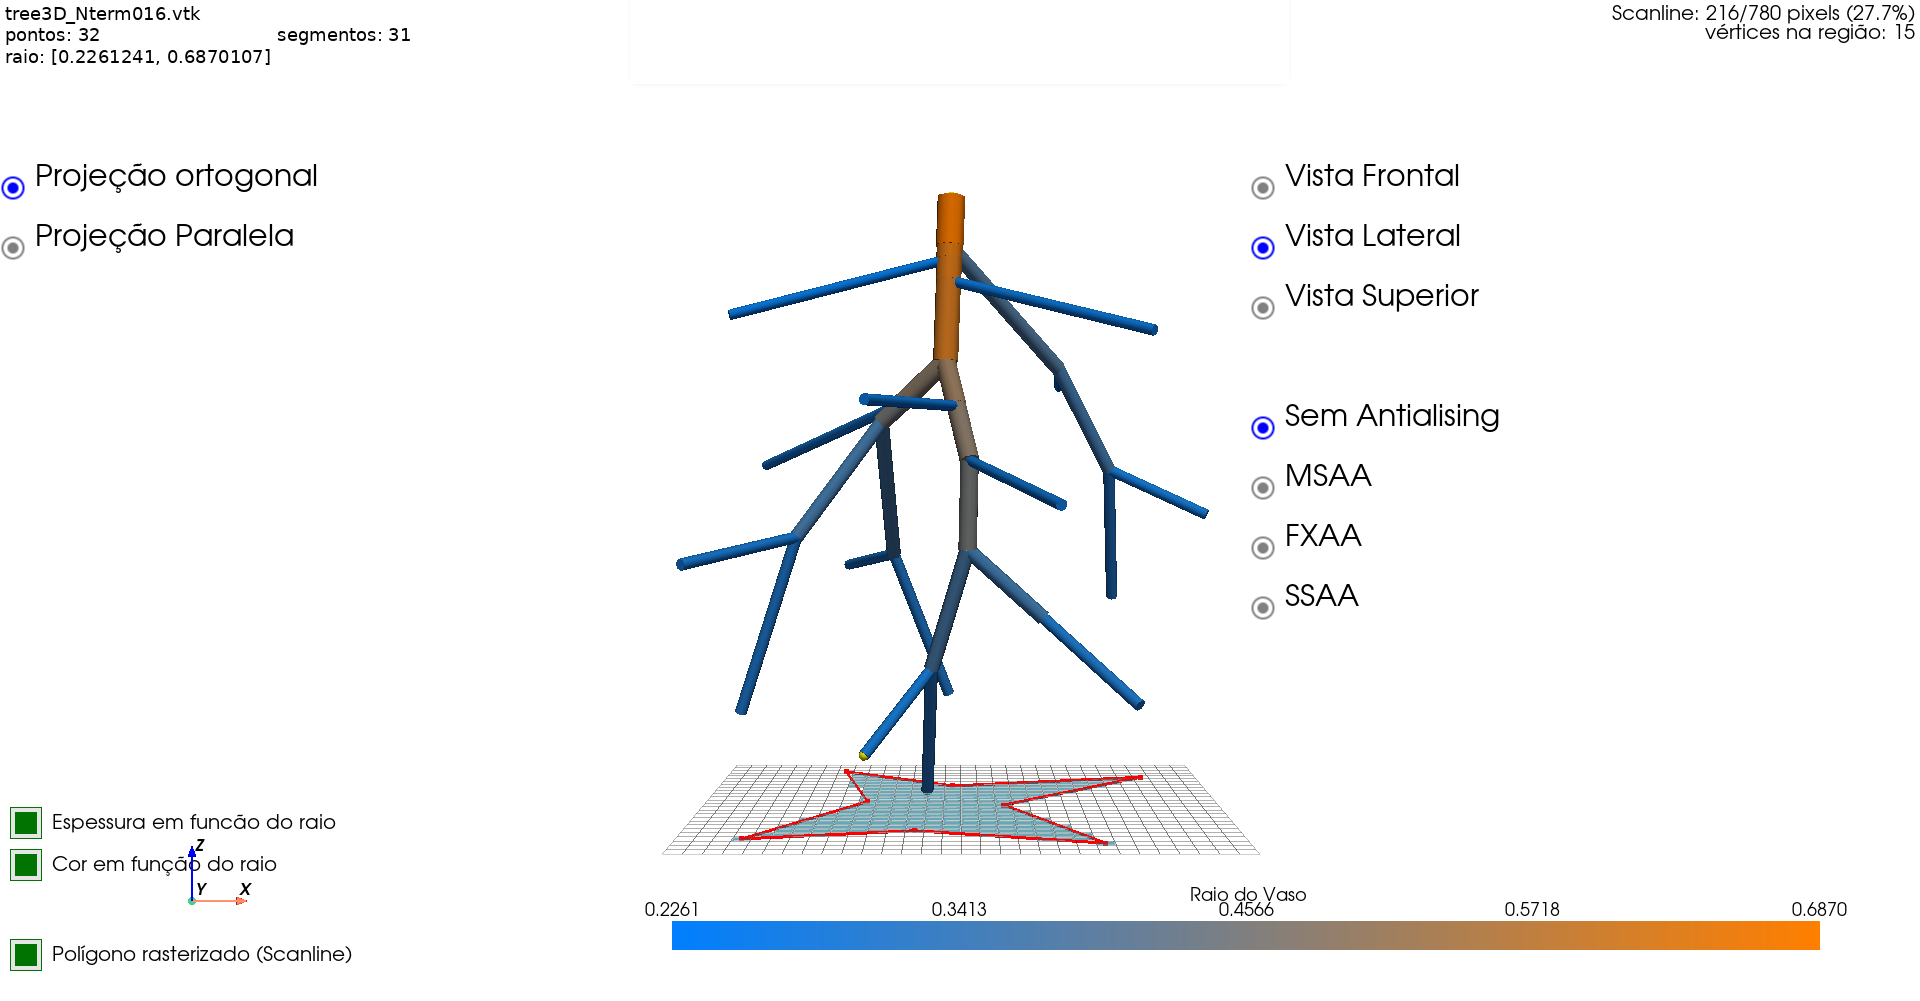
\includegraphics[width=\linewidth]{figures/aa_sem.png}
        \caption{Sem antialiasing}
        \label{fig:sem_antialiasing}
    \end{subfigure}
    \hfill % Adiciona espaço horizontal entre as duas figuras
    \begin{subfigure}{0.48\textwidth}
        \centering
        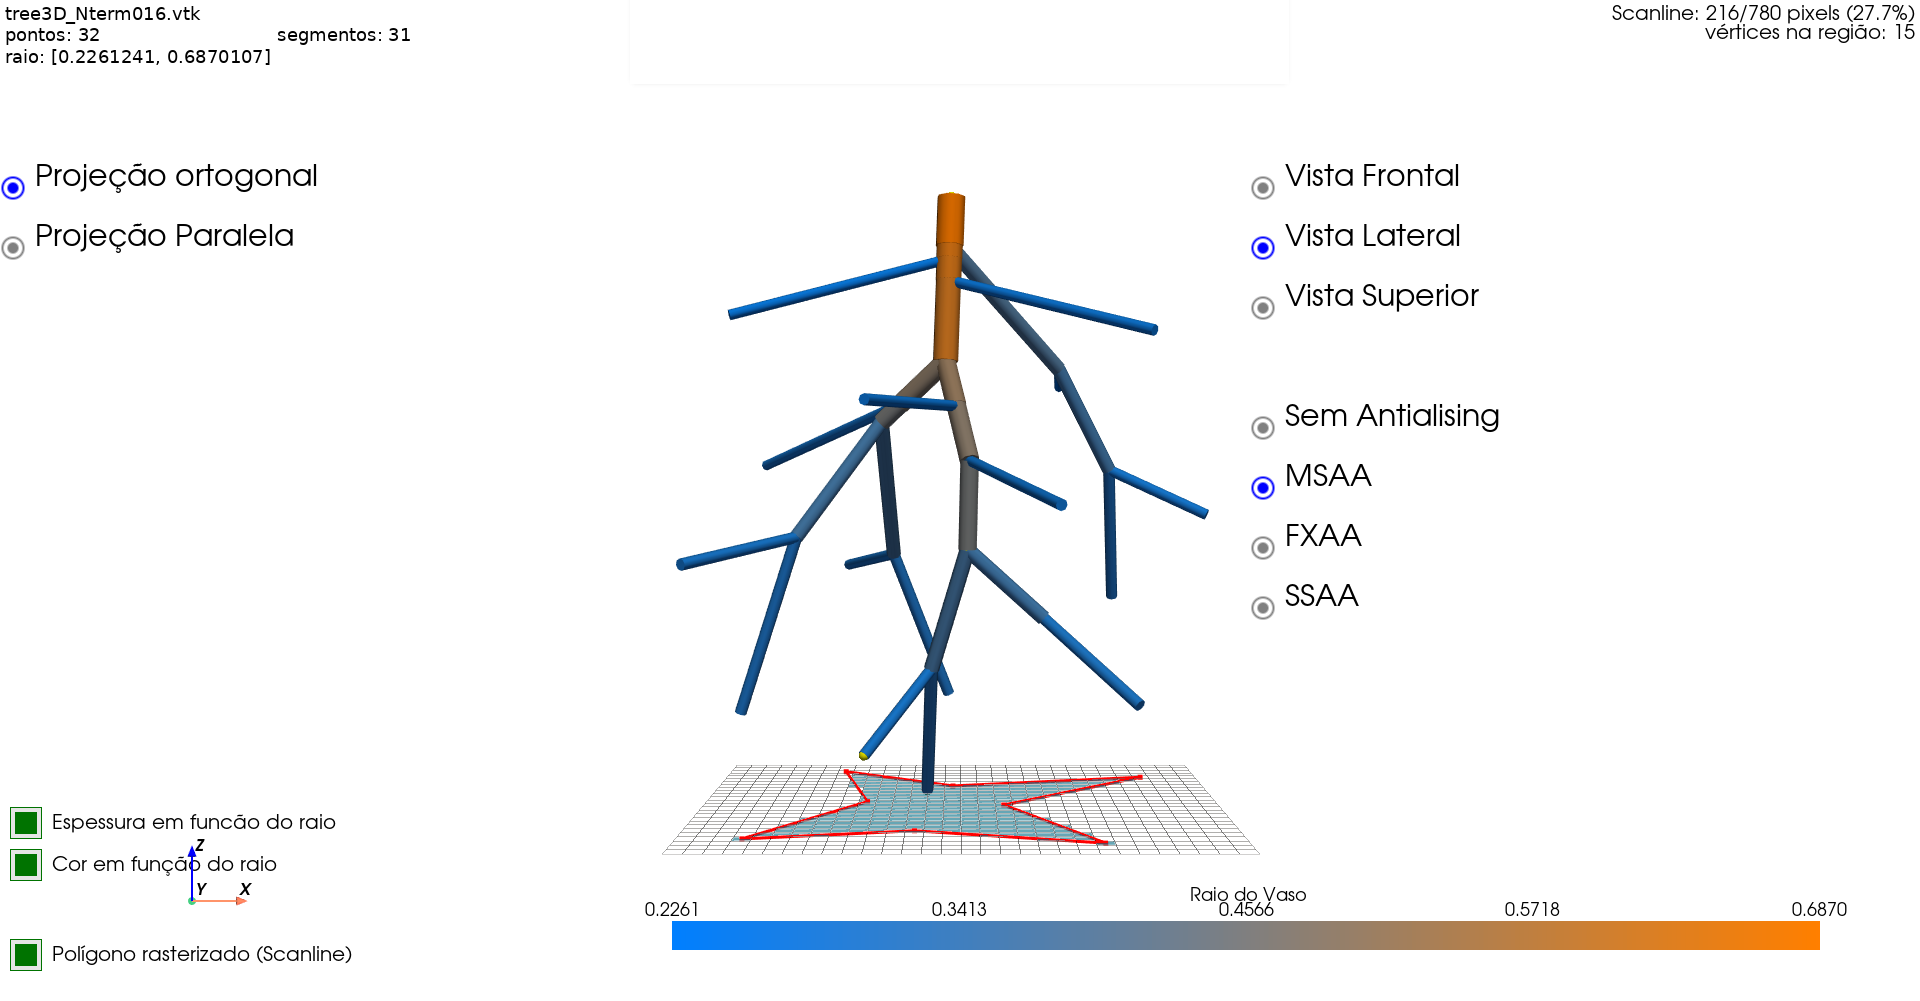
\includegraphics[width=\linewidth]{figures/aa_msaa.png}
        \caption{MSAA.}
        \label{fig:msaa}
    \end{subfigure}

    \vspace{1em} % Espaço vertical entre a primeira e a segunda linha

    % --- Segunda linha ---
    \begin{subfigure}{0.48\textwidth}
        \centering
        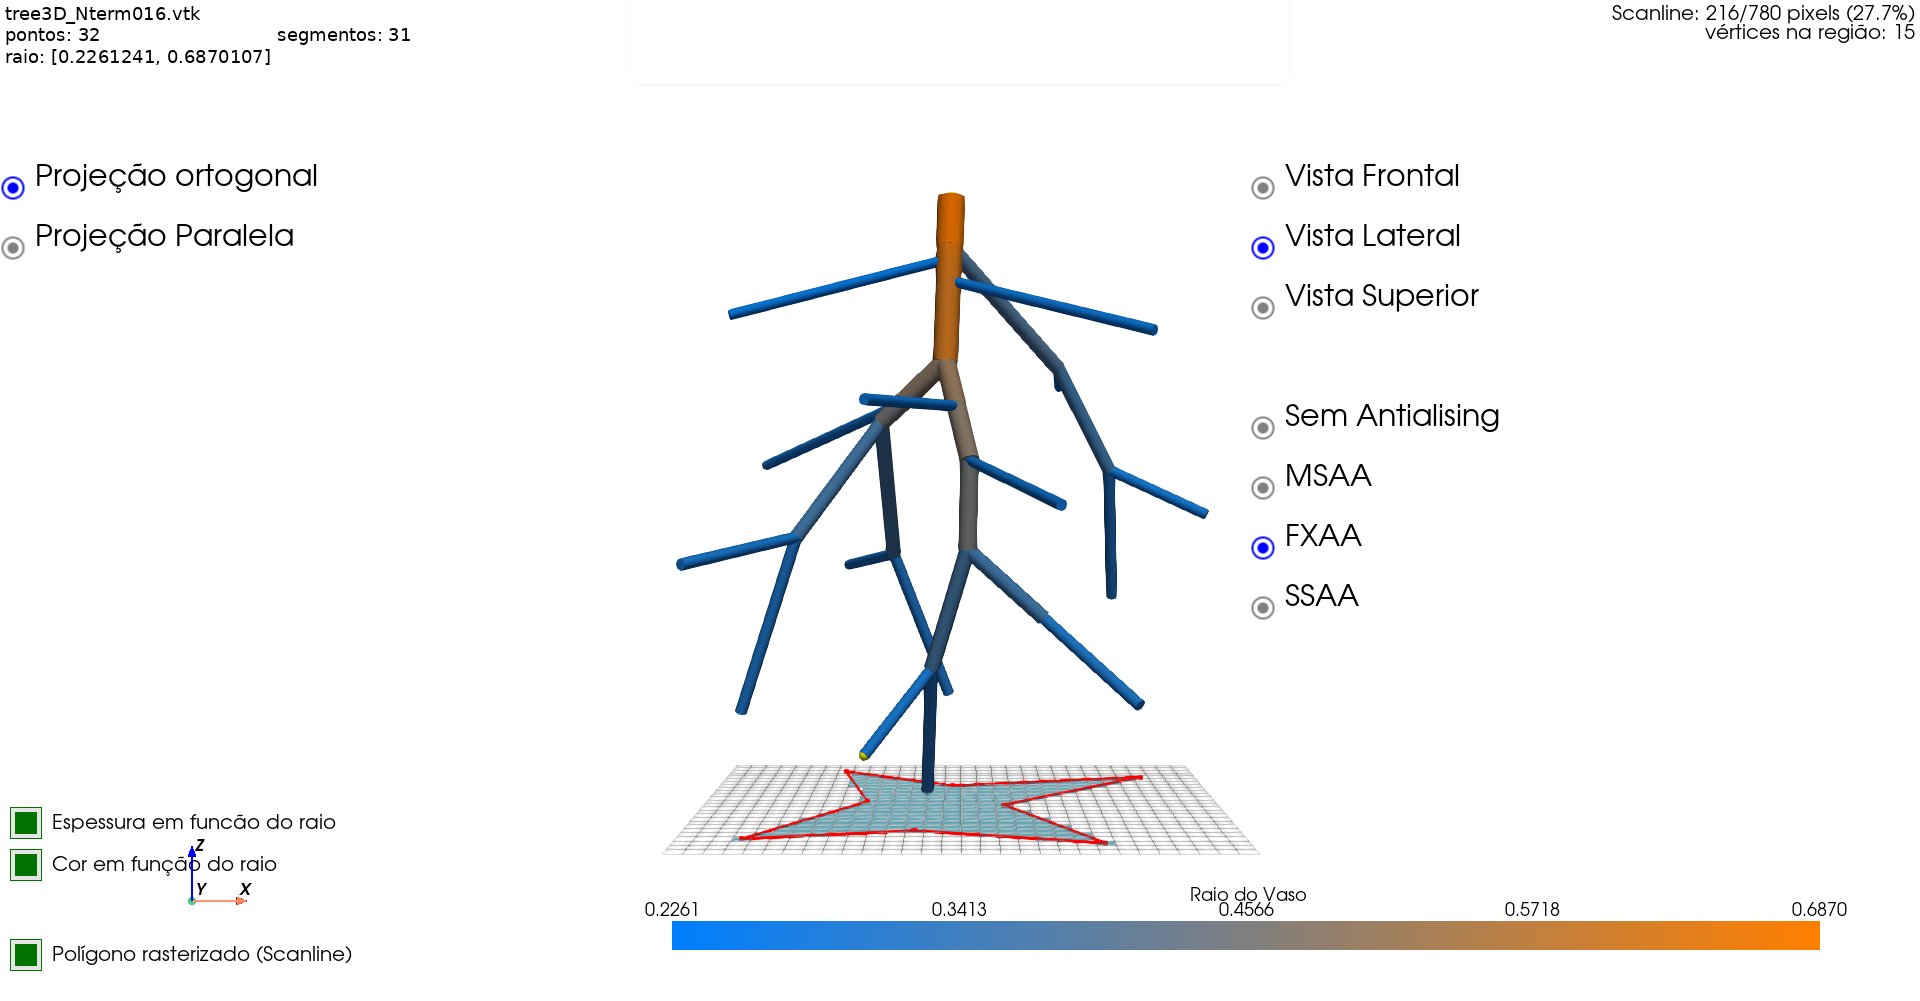
\includegraphics[width=\linewidth]{figures/aa_fxaa.png}
        \caption{FXAA.}
        \label{fig:fxaa}
    \end{subfigure}
    \hfill
    \begin{subfigure}{0.48\textwidth}
        \centering
        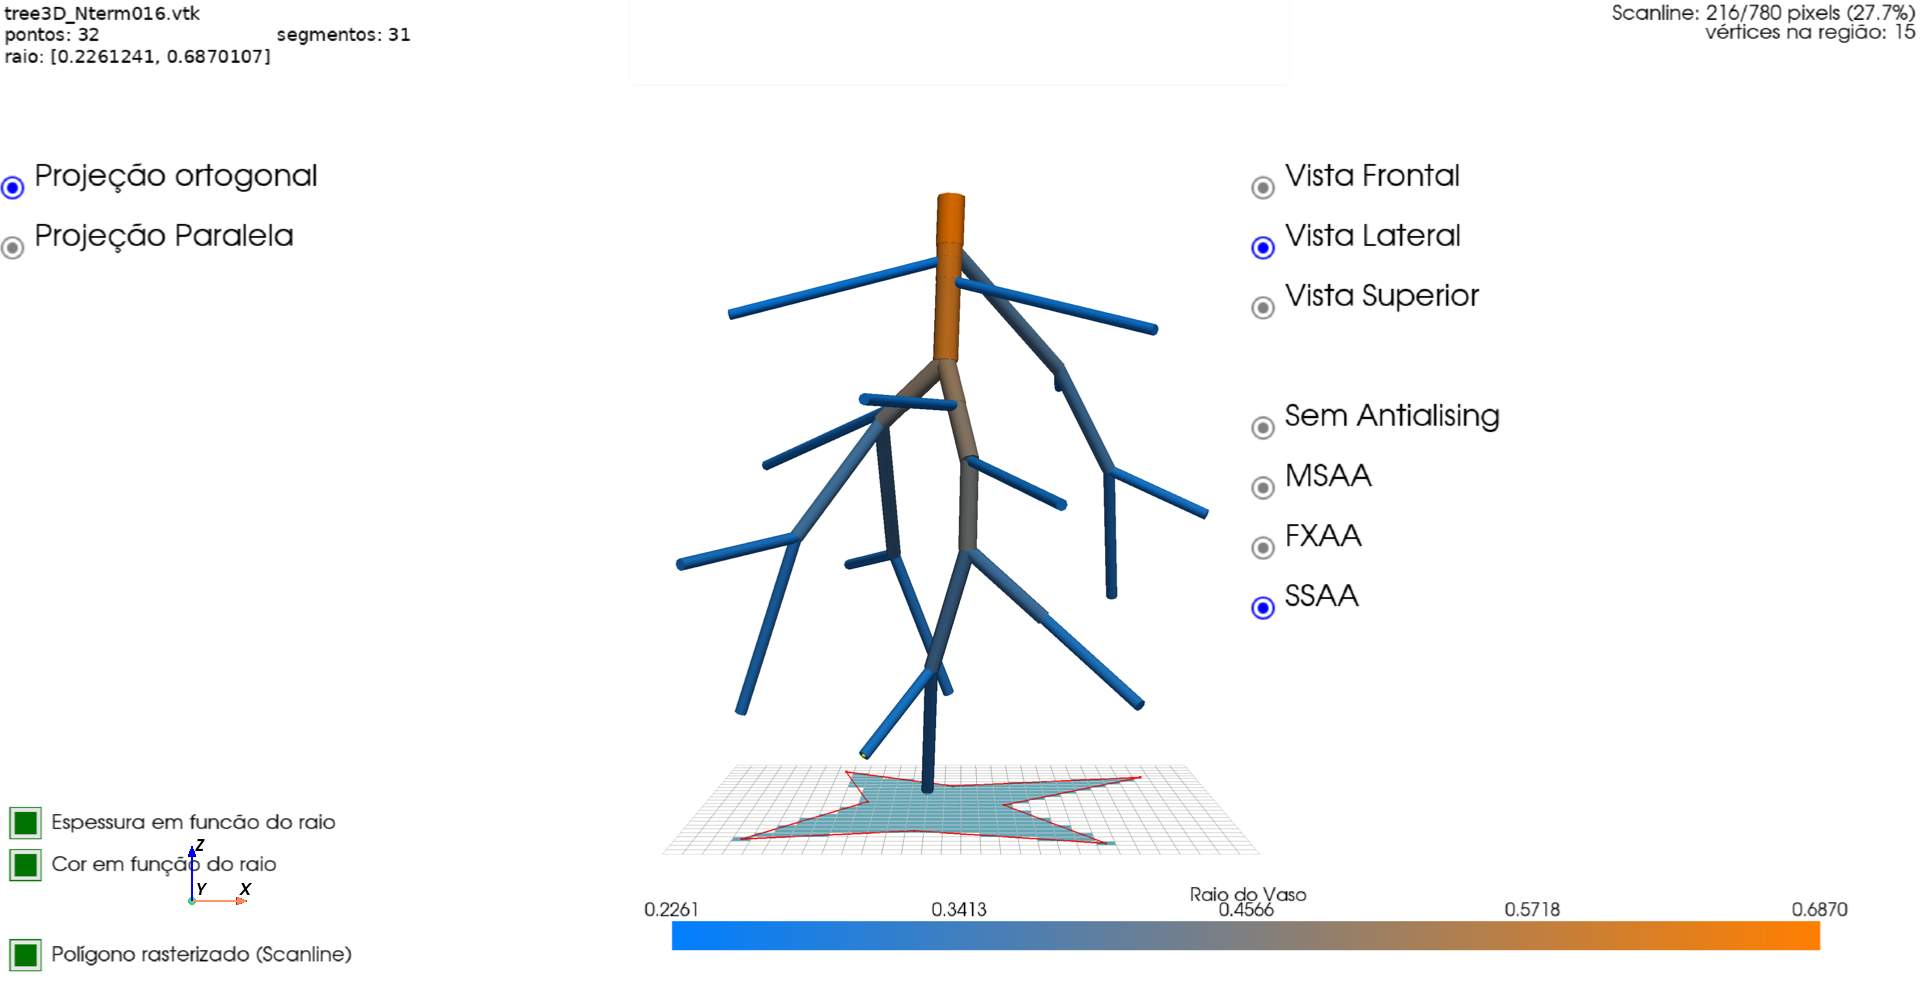
\includegraphics[width=\linewidth]{figures/aa_ssaa.png}
        \caption{SSAA.}
        \label{fig:ssaa}
    \end{subfigure}

    \caption{Comparação das diferentes configurações de Antialiasing.}
    \label{fig:comparacao_arvores_antiliasing}
\end{figure}

\subsection{Recorte de segmentos}

A Tabela~\ref{tab:clip} compara os algoritmos para a janela com fator de 50\% do tamanho da árvore para o modelo tree2D\_Nterm128.vtk. E a Figura \ref{fig:comparacao_recorte_linha} mostra visualmente a comparação da execução dos algoritmos.

\begin{table}[!h]
  \centering\small
  \caption{Estatísticas do recorte, obtidas dos contadores da aplicação.}
  \label{tab:clip}
  \begin{tabular}{|l|c|c|c|c|c|}
    \toprule
    \textbf{Algoritmo} & \textbf{Segmentos} & \textbf{Dentros} & \textbf{Cortados} & \textbf{Rejeitados} & \textbf{Interseções / Divisões} \\
    \midrule
    Cohen-Sutherland & 255 & 71 & 21 & 163 & 21 / 21\\
    Liang-Barsky & 255 & 53 & 39 & 163 & 0 / 733\\
    \bottomrule
  \end{tabular}
\end{table}

\begin{figure}[H]
    \centering
    \begin{subfigure}{0.48\textwidth}
        \centering
        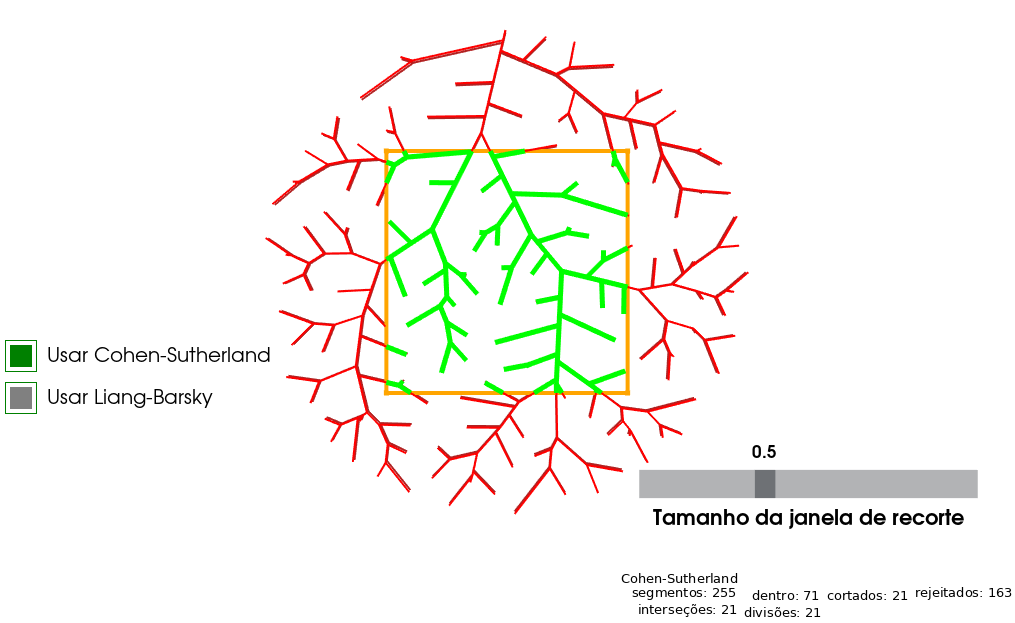
\includegraphics[width=\linewidth]{figures/cohen.png}
        \caption{Execução do algoritmo Cohen-Sutherland.}
        \label{fig:rasteriza2D}
    \end{subfigure}
    \hfill % Adiciona espaço horizontal entre as duas figuras
    \begin{subfigure}{0.48\textwidth}
        \centering
        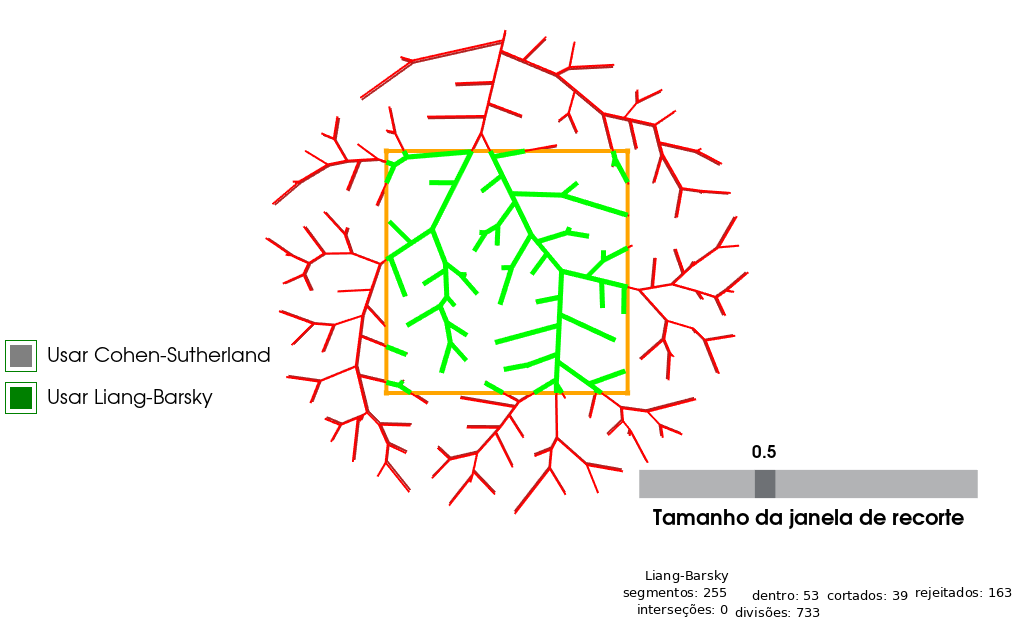
\includegraphics[width=\linewidth]{figures/liang.png}
        \caption{Execução do algoritmo Liang-Barsky.}
        \label{fig:rasteriza3D}
    \end{subfigure}

    \caption{Comparação da execução dos algoritmos Cohen-Sutherland e Liang-Barsky.}
    \label{fig:comparacao_recorte_linha}
\end{figure}

\subsection{Recorte de polígonos}

Na Figura \ref{fig:recortePoligono} mostra o resultado da execução do algoritmo Sutherland-Hodgamn no recorte de polígonos.

\begin{figure}[H]
    \centering
    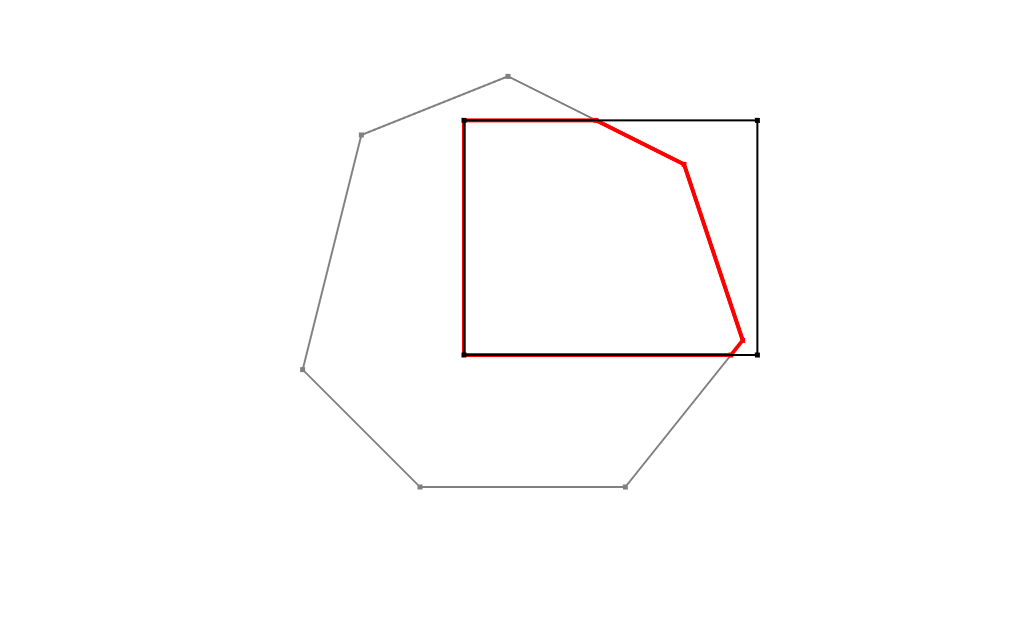
\includegraphics[width=0.75\linewidth]{figures/rasterizaçãoPoligoino.png}
    \caption{Recorte de Polígono.}
    \label{fig:recortePoligono}
\end{figure}

\section{Discussão}

Os resultados demonstram a integração de diferentes conceitos em uma aplicação única. O módulo 1 realiza a interpretação do arquivo VTK e constrói uma representação tubular que torna a estrutura vascular mais legível. A codificação do raio por cor e espessura amplia a quantidade de informação visual sem modificar a geometria topológica de entrada. O módulo 4 constitui a parte algorítmica mais explícita: o preenchimento é calculado em código próprio, com tabela de arestas e atualização incremental das interseções, em vez de ser delegado integralmente ao renderizador.

Há, entretanto, diferenças importantes entre os requisitos do enunciado e o estado atual do programa. O módulo 2 permite escolher vistas e alternar a projeção por meio da API, mas não implementa operações explícitas de translação, rotação e escala do objeto. A interface também apresenta os rótulos das projeções invertidos em relação às chamadas da câmera.


\subsection{Implementado pelo grupo × auxílio da biblioteca}
A Tabela~\ref{tab:atribuicao} separa explicitamente as partes.

\begin{table}[htbp]
  \centering\small
  \caption{Divisão entre o que foi implementado pelo grupo e o que foi fornecido pelo PyVista/VTK.}
  \label{tab:atribuicao}
  \begin{tabularx}{\textwidth}{l X X}
    \toprule
    \textbf{Tópico} & \textbf{Implementado pelo grupo} & \textbf{Auxílio de biblioteca}\\
    \midrule
    1. Leitura/atributos & Decomposição em segmentos, detecção do raio, mapa de cor, escala de espessura & Leitura do VTK; filtro de tubos\\
    2. Observador & Organização de vistas e botões & Câmera, matrizes de visão e projeção, interação\\
    3. Linhas & DDA e Bresenham & Figura com Matplotlib\\
    4. Polígonos & Scanline (ET/AET), geometria dos retângulos, projeção, rotação & Exibição do buffer como malha de pixels\\
    5. Antialiasing & Interface de seleção e comparação & MSAA, FXAA e SSAA\\
    6. Recorte de segmentos & Cohen-Sutherland, Liang-Barsky, interpolação de $z$, contadores & Exibição das linhas\\
    7. Recorte de polígonos & Sutherland-Hodgman (quatro bordas, histórico por etapa), polígono de teste, arraste da janela & Janela 2D, câmera paralela, eventos de mouse (VTK)\\
    \bottomrule
  \end{tabularx}
\end{table}

\subsection{Comparação entre os algoritmos de recorte}
Cohen-Sutherland é eficiente quando a maioria dos segmentos é trivialmente aceita ou rejeitada, mas, para segmentos que cruzam a janela, pode recalcular interseções e códigos por até quatro iterações, cada uma com uma divisão. Liang-Barsky calcula no máximo quatro razões $q_k/p_k$ e só obtém os pontos recortados uma vez ao final, evitando interseções intermediárias. Cyrus-Beck, não implementado, usa a mesma ideia paramétrica, mas aceita qualquer janela convexa, ao custo de produtos escalares em vez de simples diferenças de coordenadas.

\subsection{Sutherland-Hodgman e Weiler-Atherton}
Sutherland-Hodgman funciona com qualquer polígono contra uma janela convexa, mas, ao recortar polígonos côncavos, pode produzir arestas degeneradas (sobrepostas) ao ligar partes que deveriam ser regiões separadas, pois sua saída é sempre uma única lista de vértices. O Weiler-Atherton~\cite{weileratherton1977} é mais adequado quando há polígonos côncavos, quando a interseção gera múltiplas regiões disjuntas e quando a janela também é um polígono arbitrário, incluindo côncavo ou com buracos: ao percorrer as listas de entrada e saída, ele separa corretamente as regiões resultantes. Em contrapartida, é bem mais complexo de implementar.

\subsection{Decisões de implementação e limitações}
\begin{itemize}[leftmargin=*]
  \item O mapa de cores RGB linear é simples, mas não é perceptualmente uniforme; mapas contínuos como o \emph{viridis} facilitariam a leitura de diferenças sutis de raio.
  \item No DDA, a função \texttt{round} de Python arredonda valores intermediários ($x{,}5$) para o inteiro par mais próximo, o que pode gerar pequenas diferenças em relação ao Bresenham.
  \item O Módulo 3 rasteriza apenas os 20 primeiros segmentos, por clareza visual; a fração 500 de conversão para inteiros depende da escala do modelo.
  \item O recorte do Módulo 6 considera apenas o plano $xy$ (com interpolação de $z$); não há recorte volumétrico em 3D.
  \item No Módulo 4, a ordenação por profundidade é uma aproximação (algoritmo do pintor) e não substitui um Z-buffer.
  \item No Módulo 7, a janela só pode ser arrastada (tamanho fixo), a interface demonstra apenas o polígono convexo (o côncavo foi testado por chamada direta da função) e o módulo abre janela própria.
  \item O Sutherland-Hodgman implementado serve apenas a janelas retangulares alinhadas aos eixos e não separa regiões disjuntas.
\end{itemize}

\section{Conclusão}
Este trabalho resultou em uma aplicação modular que integra leitura, visualização, rasterização, antialiasing e recorte de modelos de árvores arteriais CCO. Os algoritmos clássicos solicitados (DDA e Bresenham, Scanline, Cohen-Sutherland, Liang-Barsky e Sutherland-Hodgman) foram implementados diretamente pelo grupo, enquanto a leitura dos arquivos, a renderização, a câmera e o antialiasing ficaram a cargo do PyVista/VTK, como documentado na Tabela~\ref{tab:atribuicao}.

Os experimentos permitiram observar, de forma concreta, o que os livros descrevem: DDA e Bresenham geram praticamente os mesmos pixels com custos diferentes; Cohen-Sutherland e Liang-Barsky recortam igualmente os segmentos, mas com quantidades distintas de interseções e divisões; e o Sutherland-Hodgman é simples e correto para polígonos convexos, mas não representa corretamente a saída quando o recorte de um polígono côncavo produz mais de uma região. O trabalho também deixou claro o contraste entre algoritmos didáticos e o pipeline gráfico, que realiza essas etapas em hardware.

\section*{Agradecimentos}
Os autores agradecem ao Departamento de Computação (DECOM) e à Universidade Federal de Ouro Preto (UFOP) pela infraestrutura e ao Prof.\ Rafael Alves Bonfim de Queiroz pelo material, aulas e pelos modelos CCO fornecidos.

\newpage
\sloppy
\begin{thebibliography}{9}

\bibitem{schreiner1993}
SCHREINER, W.; BUXBAUM, P.
Computer-optimization of vascular trees.
\textit{IEEE Transactions on Biomedical Engineering}, v. 40, n. 5, p. 482--491, 1993.

\bibitem{foley1996}
FOLEY, J. D.; VAN DAM, A.; FEINER, S. K.; HUGHES, J. F.
\textit{Computer Graphics: Principles and Practice}.
2. ed. Reading: Addison-Wesley, 1996.

\bibitem{pyvista}
PYVISTA DEVELOPERS.
\textit{PyVista Documentation}.
Disponível em: \url{https://docs.pyvista.org/}. Acesso em: 11 nov. 2026.

\bibitem{vtk}
KITWARE.
\textit{VTK -- The Visualization Toolkit}.
Disponível em: \url{https://vtk.org/}. Acesso em: 11 nov. 2026.


\bibitem{bresenham1965} BRESENHAM, J. E. Algorithm for computer control of a digital plotter. \textbf{IBM Systems Journal}, v. 4, n. 1, p. 25--30, 1965.

\bibitem{liangbarsky1984} LIANG, Y.-D.; BARSKY, B. A. A new concept and method for line clipping. \textbf{ACM Transactions on Graphics}, v. 3, n. 1, p. 1--22, 1984.
  
\bibitem{cyrusbeck1978} CYRUS, M.; BECK, J. Generalized two- and three-dimensional clipping. \textbf{Computers \& Graphics}, v. 3, n. 1, p. 23--28, 1978.
  
\bibitem{sutherlandhodgman1974} SUTHERLAND, I. E.; HODGMAN, G. W. Reentrant polygon clipping. \textbf{Communications of the ACM}, v. 17, n. 1, p. 32--42, 1974.

\bibitem{weileratherton1977} WEILER, K.; ATHERTON, P. Hidden surface removal using polygon area sorting. In: \textbf{SIGGRAPH '77}, p. 214--222, 1977.

\end{thebibliography}

\end{document}
